\todo{There should be a link either here or at end of literature which forms the basic for different methods (clustering, routing, trip generation).}
\todo{Brief Paragraph describing different types of algorithm used (Routing then cluster, Cluster then Routing, Genetic, etc.)}
\todo{Remember to justify the choice of algorithms. You may also need to explain how to adopt these algorithms in your work. A figure showing the ralationship between different components of your work may also help.}

\subsection{Implementation Pre-Requisites}\label{subsec:implementation-pre-requisites}
There are two things need before we begin, a way of generating inputs to use our algorithms on, and an
implementation of our objective function so we can evaluate our results.

\subsubsection{Input Generation}\label{subsubsec:input-generation}
For our input we will be using Openrouteservice's Points of Interest (PoI) and Distance Matrix API services.
With the PoI service, we can input a location, such as a city centre, and retrieve a specified number of locations
of interest around the area.
The PoI service also allows us to limit the locations returned to certain categories allowing us to specifically find
locations that one would likely be interested in visiting, for example points labelled 'tourism', 'historic' or
'arts and culture'.

After we have these locations, we can use the Distance Matrix to create a graph linking each location to each other
with a weight associated with travelling between them.
We can configure our API call to this service such that, instead of distance, the weights in the matrix represent
the time taken to travel between locations via public transport.
Unfortunately, the Distance Matrix service limits the number of locations in a call to 25, severely limiting the
size of input we can test.
Other alternative API's were looked into, such as the Google Maps API or Mapbox, but all the alternatives found were
either too expensive or equally, if not more, restrictive.

With these, we can generate a list of durations associated with the found locations, as well as a number of days for
the trip, and then our input is ready.

\subsubsection{Objective Function}\label{subsubsec:algorithms-objective-function}
As described in the \hyperref[sec:problem-formulation]{Problem Formulation}, our objective function aims to
calculate a cost for a given route.
This function is needed such that we can compare our approaches and algorithms based on the quality of their results.
Figure~\ref{fig:Algorithm.evaluate_route} shows how this was implemented in our project.
\begin{figure}[H]
    \centering
    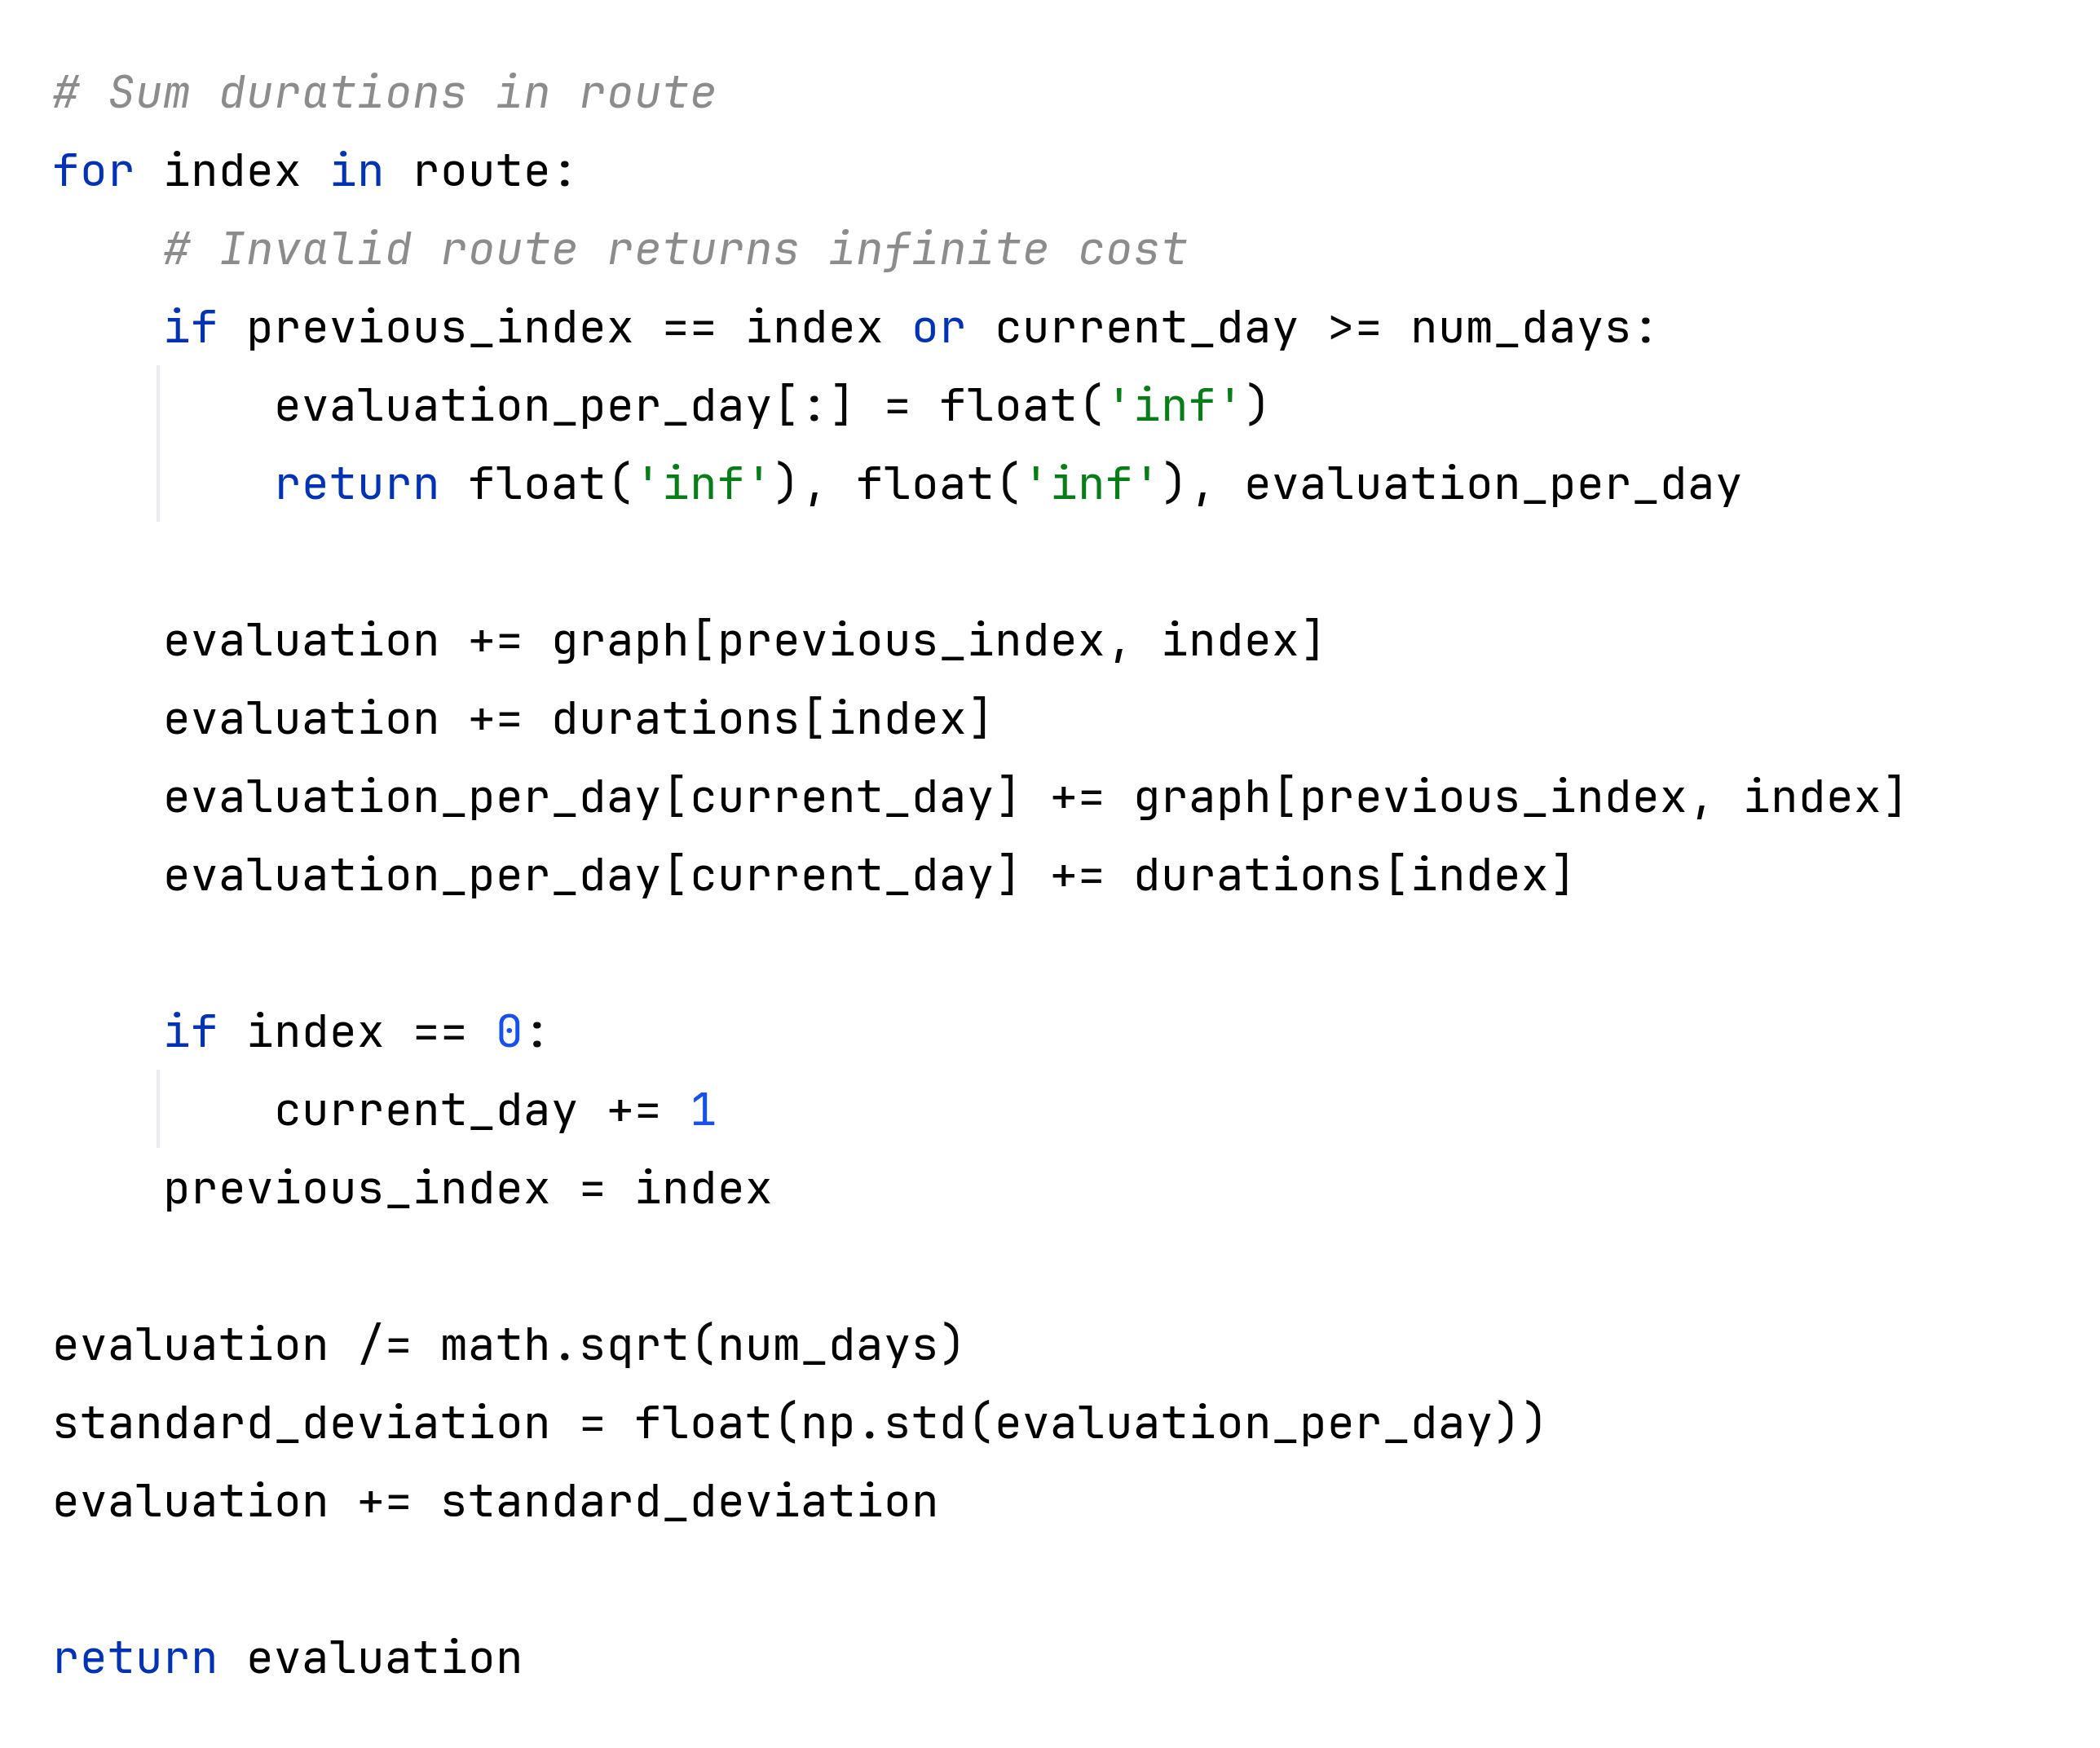
\includegraphics[width = \textwidth]{Algorithm.evaluate_route}
    \caption{Code from Algorithm.evaluate\_route in algorithms\textbackslash algorithm.py}
    \label{fig:Algorithm.evaluate_route}
\end{figure}

\subsubsection{Project Code}\label{subsubsec:project-code}
All the code used in the project is available to find at: \url{https://git.cs.bham.ac.uk/projects-2024-25/jhl114}.
Code snippets shown in this report, such as figure~\ref{fig:Algorithm.evaluate_route}, are captioned
detailing where in the git repository their code can be found.

\subsection{Clustering}\label{subsec:clustering}
Clustering as a concept can be described as `the unsupervised classification of patterns (observation, data items, or
feature vectors) into groups (clusters)'\todo{cite Data Clustering: A review, A.K. Jain}.
In our problem, clustering will be used to group locations together to form an itinerary for each day of the trip.
These clusters, or days, will then be used as an input for some routing algorithm, which will try and find an
optimal route for each day, which can then be combined to form a complete trip.
The goal of our clustering algorithms is to find a set of clusters that, when combined with some routing algorithm,
will produce a trip with minimal cost.
The code in figure~\ref{fig:Clustering.find_route_from_clusters} shows how we can use a set of clusters alongside our
graph and duration inputs to find a trip.
\begin{figure}[H]
    \centering
    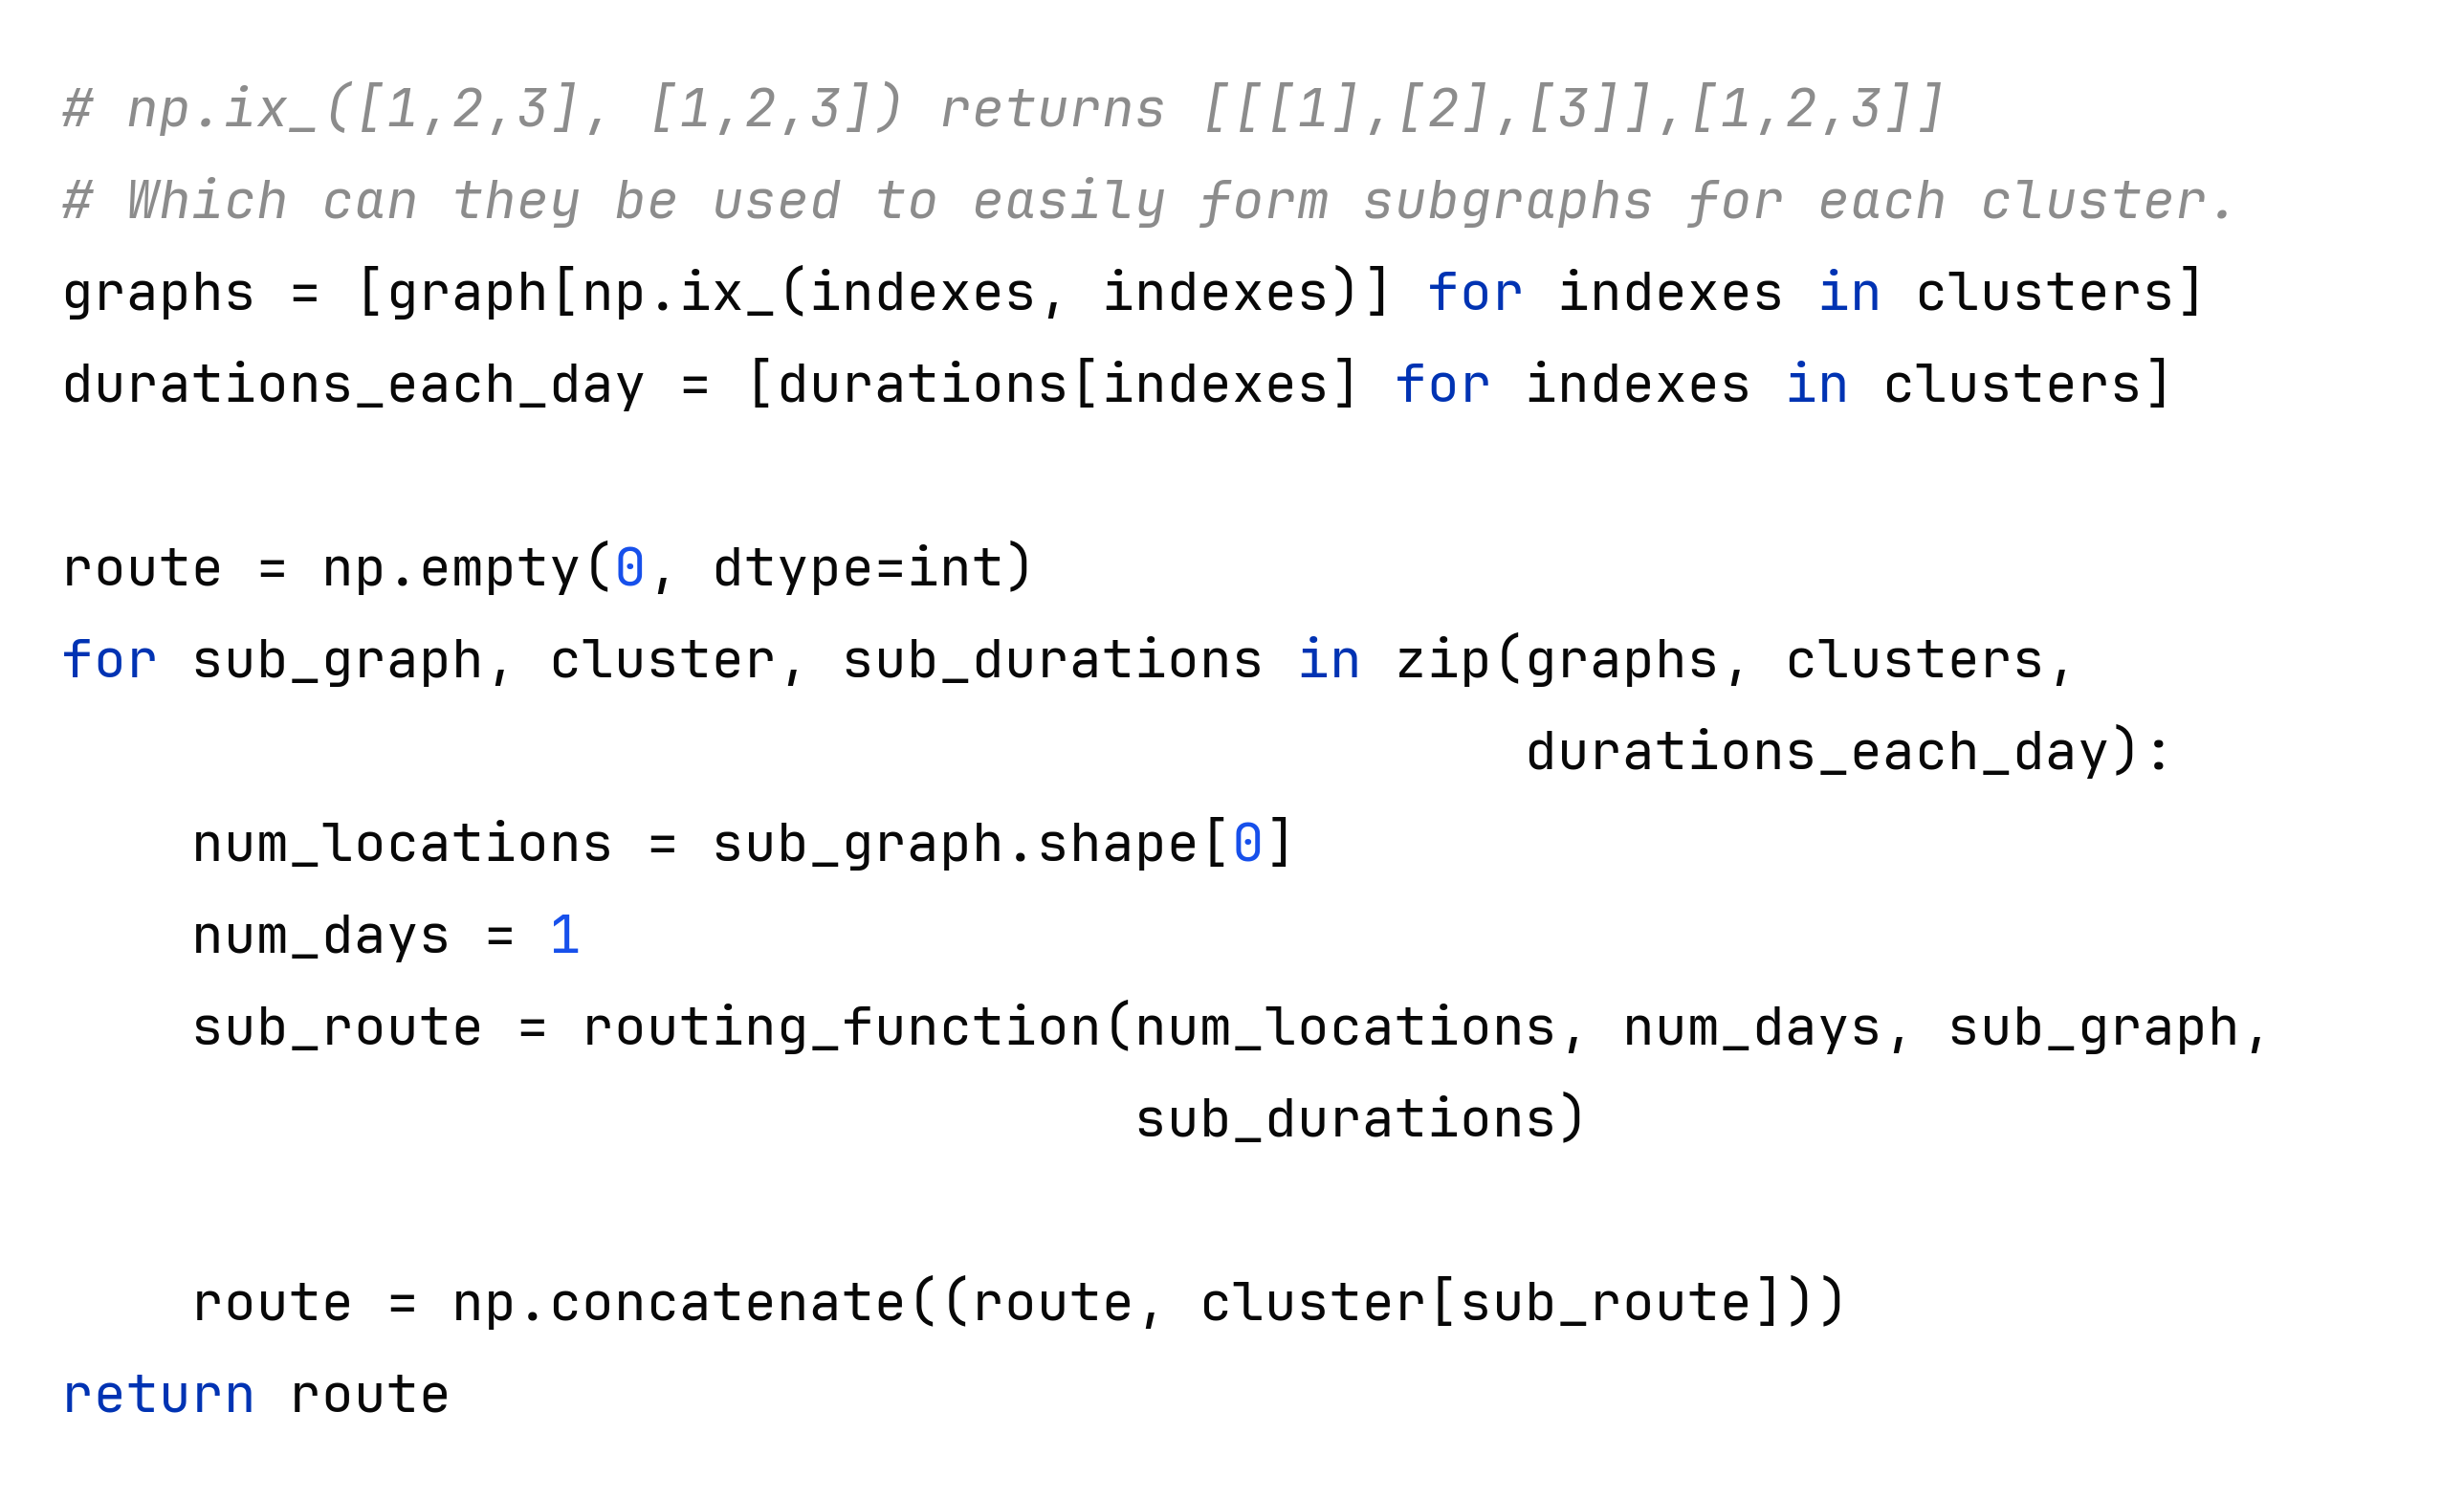
\includegraphics[width = \textwidth]{Clustering.find_route_from_clusters}
    \caption{Code from Clustering.find\_route\_from\_clusters in algorithms\textbackslash clustering.py}
    \label{fig:Clustering.find_route_from_clusters}
\end{figure}

\noindent
The clustering algorithms implemented in this project are: K-Means, Genetic Clustering and Genetic Centroid-based
Clustering.

\subsubsection{K-Means}\label{subsubsec:k-means}
K-Means is an iterative clustering algorithm that defines its clusters using a set of centroids (means) which are
given a location in the input space, a given location is assigned to the cluster of the `closest' centroid.
The algorithm starts by initialising random centroids and iteratively improving the clustering from there, continuing
until the algorithm converges (on a local optimum) or an iteration limit is reached.
K-Means runs in linear time with a time complexity of $O(m n k i)$, where $m$ is the number of locations, $n$ is the
dimensionality of the input, $k$ is the number of clusters, and $i$ is the number of iterations
\todo{cite Algorithm AS 136: A K-Means Clustering Algorithm}.
Our inputs will always contain only two dimensions, and we will be setting a maximum number of iterations, this
makes both $n$ and $i$ constants allowing us to simplify the time complexity to $O(m k)$.\\

\noindent
In our implementation of K-Means we will initialise our centroids by randomly selecting unique locations from our
input, and placing our centroids at their coordinates.
A different approach was considered, which involved initialising the centroids with random coordinates in a similar
area to the input, however this had the potential to create clusters with zero locations assigned to them resulting
in invalid trips.
By starting with locations from the input, we can be sure that all clusters have at least one location assigned to them.
We will be using the coordinates of our locations to calculate the Euclidean distances between locations and centroids,
these locations will be assigned to the cluster of the closest centroid.
Figure~\ref{fig:Clustering._assign_nodes_to_centroid} shows how this was accomplished.
\begin{figure}[H]
    \centering
    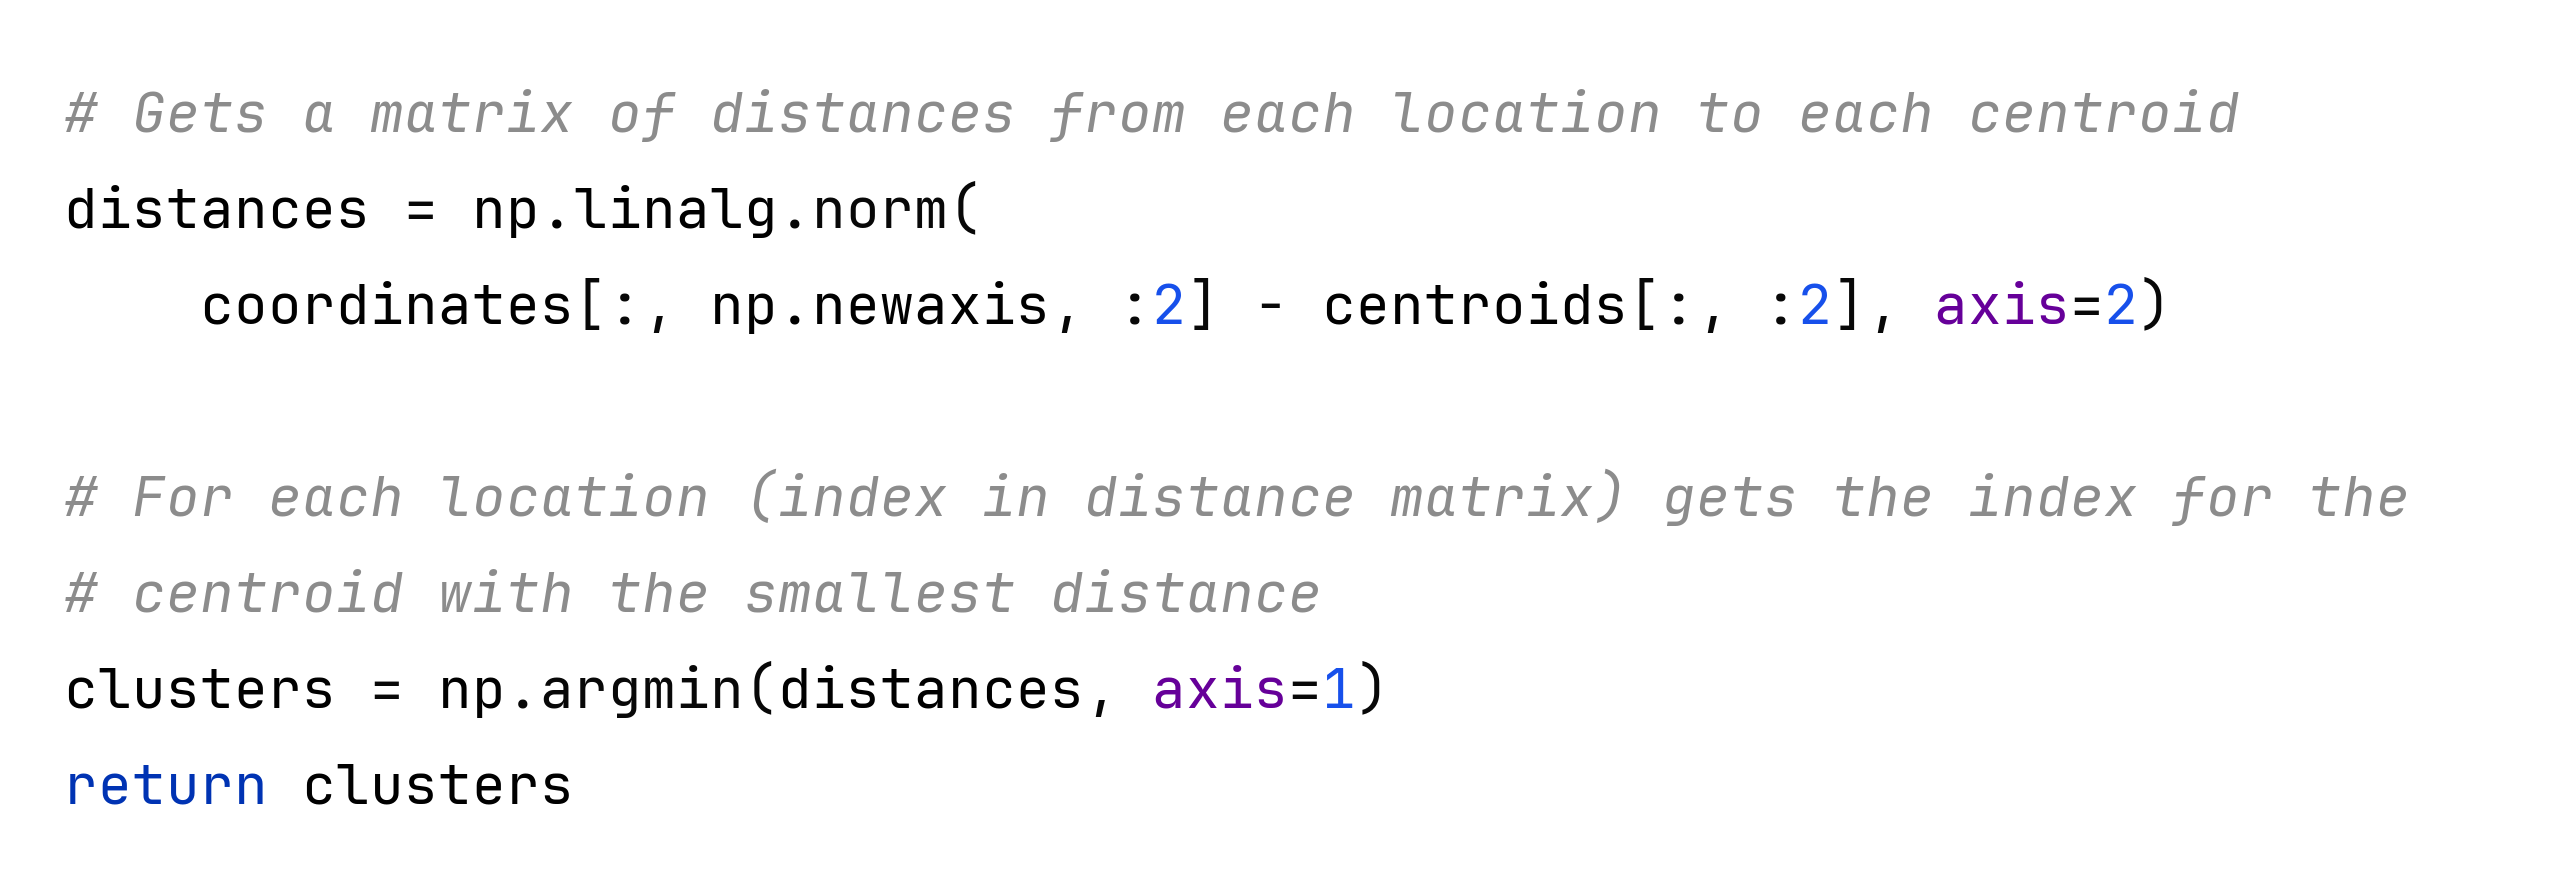
\includegraphics[width = \textwidth]{Clustering._assign_nodes_to_centroid}
    \caption{Code from Clustering.\_assign\_nodes\_to\_centroid in algorithms\textbackslash clustering.py}
    \label{fig:Clustering._assign_nodes_to_centroid}
\end{figure}

\noindent
After assignment, the centroids are recalculated such that their coordinates are the average of all locations
assigned to their cluster.
This is done by iterating through each cluster and calculating the mean of all locations assigned to it.
Our implementation is shown in figure~\ref{fig:KMeans._compute_means}.
\begin{figure}[H]
    \centering
    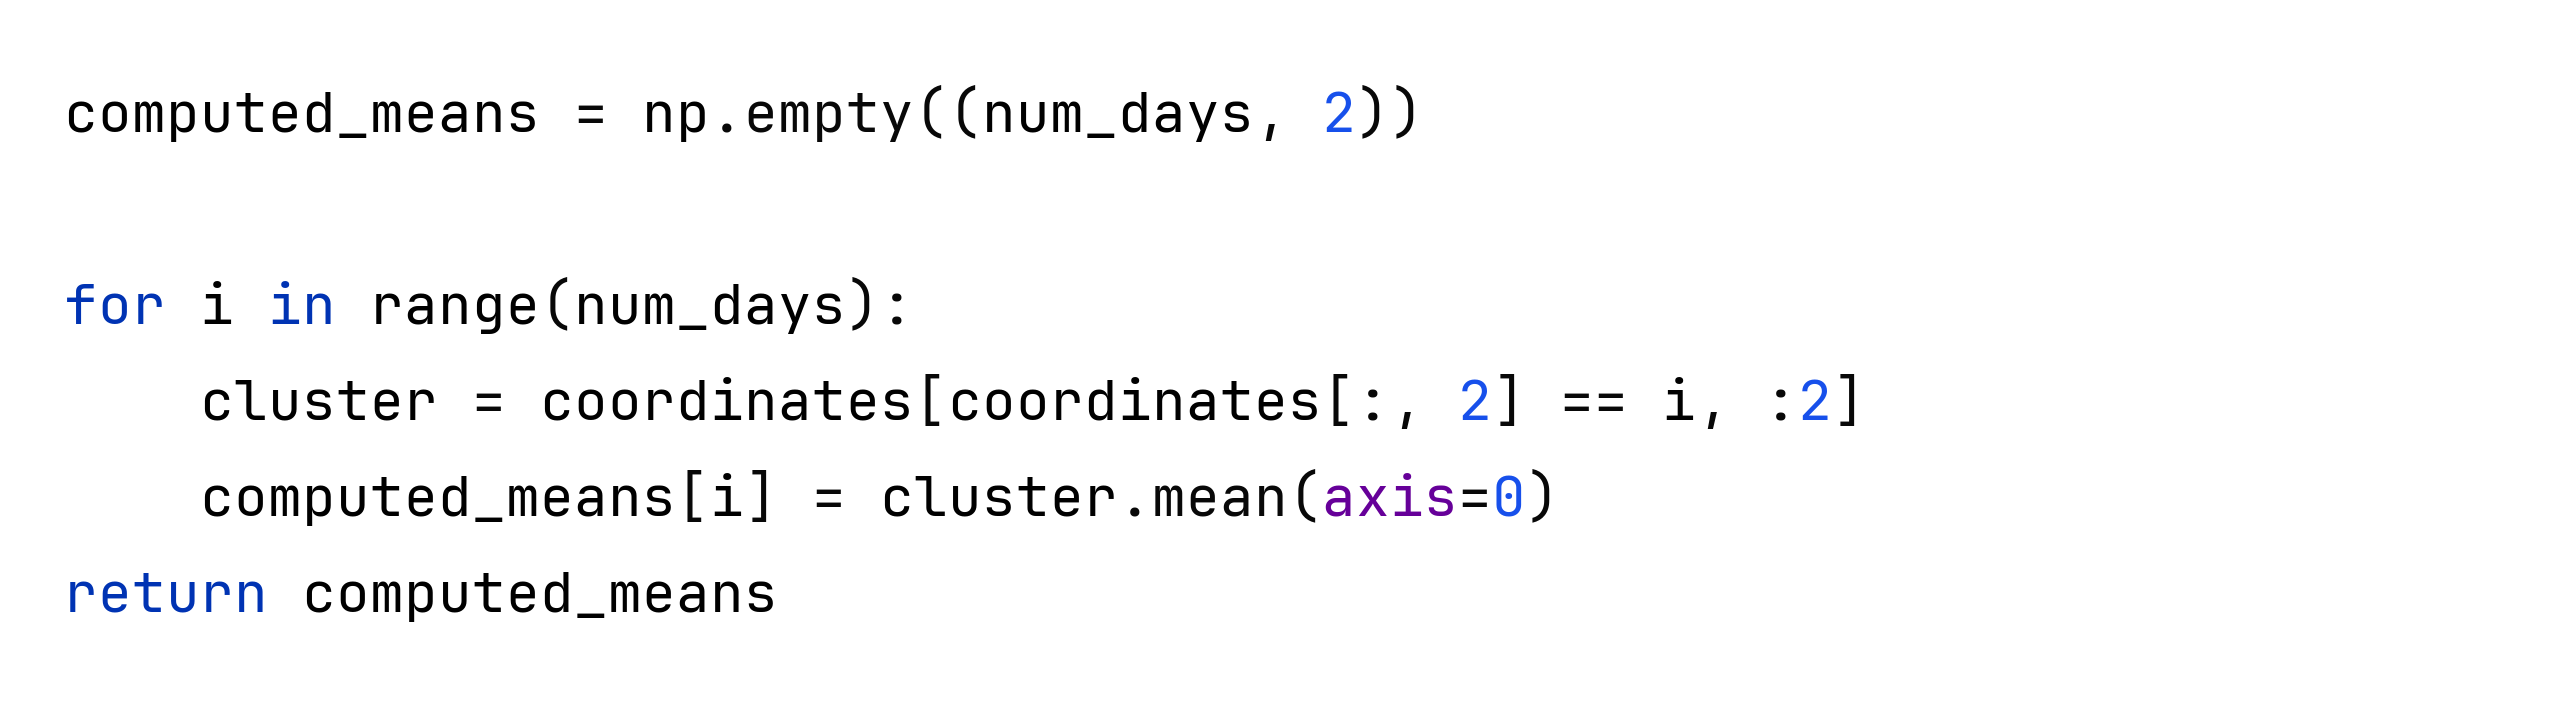
\includegraphics[width = \textwidth]{KMeans._compute_means}
    \caption{Code from KMeans.\_compute\_means in algorithms\textbackslash clustering.py}
    \label{fig:KMeans._compute_means}
\end{figure}

\noindent
These steps of cluster assignment and centroid recalculation are repeated until either a maximum allowed number of
iterations is reached, or until the algorithm converges on an optimum solution.
Our convergence criterion is that the centroids stop changing between iterations, i.e., the centroids are the same
as the previous iteration.
Our python implementation of this is shown in figure~\ref{fig:KMeans.find_clusters}.
\begin{figure}[H]
    \centering
    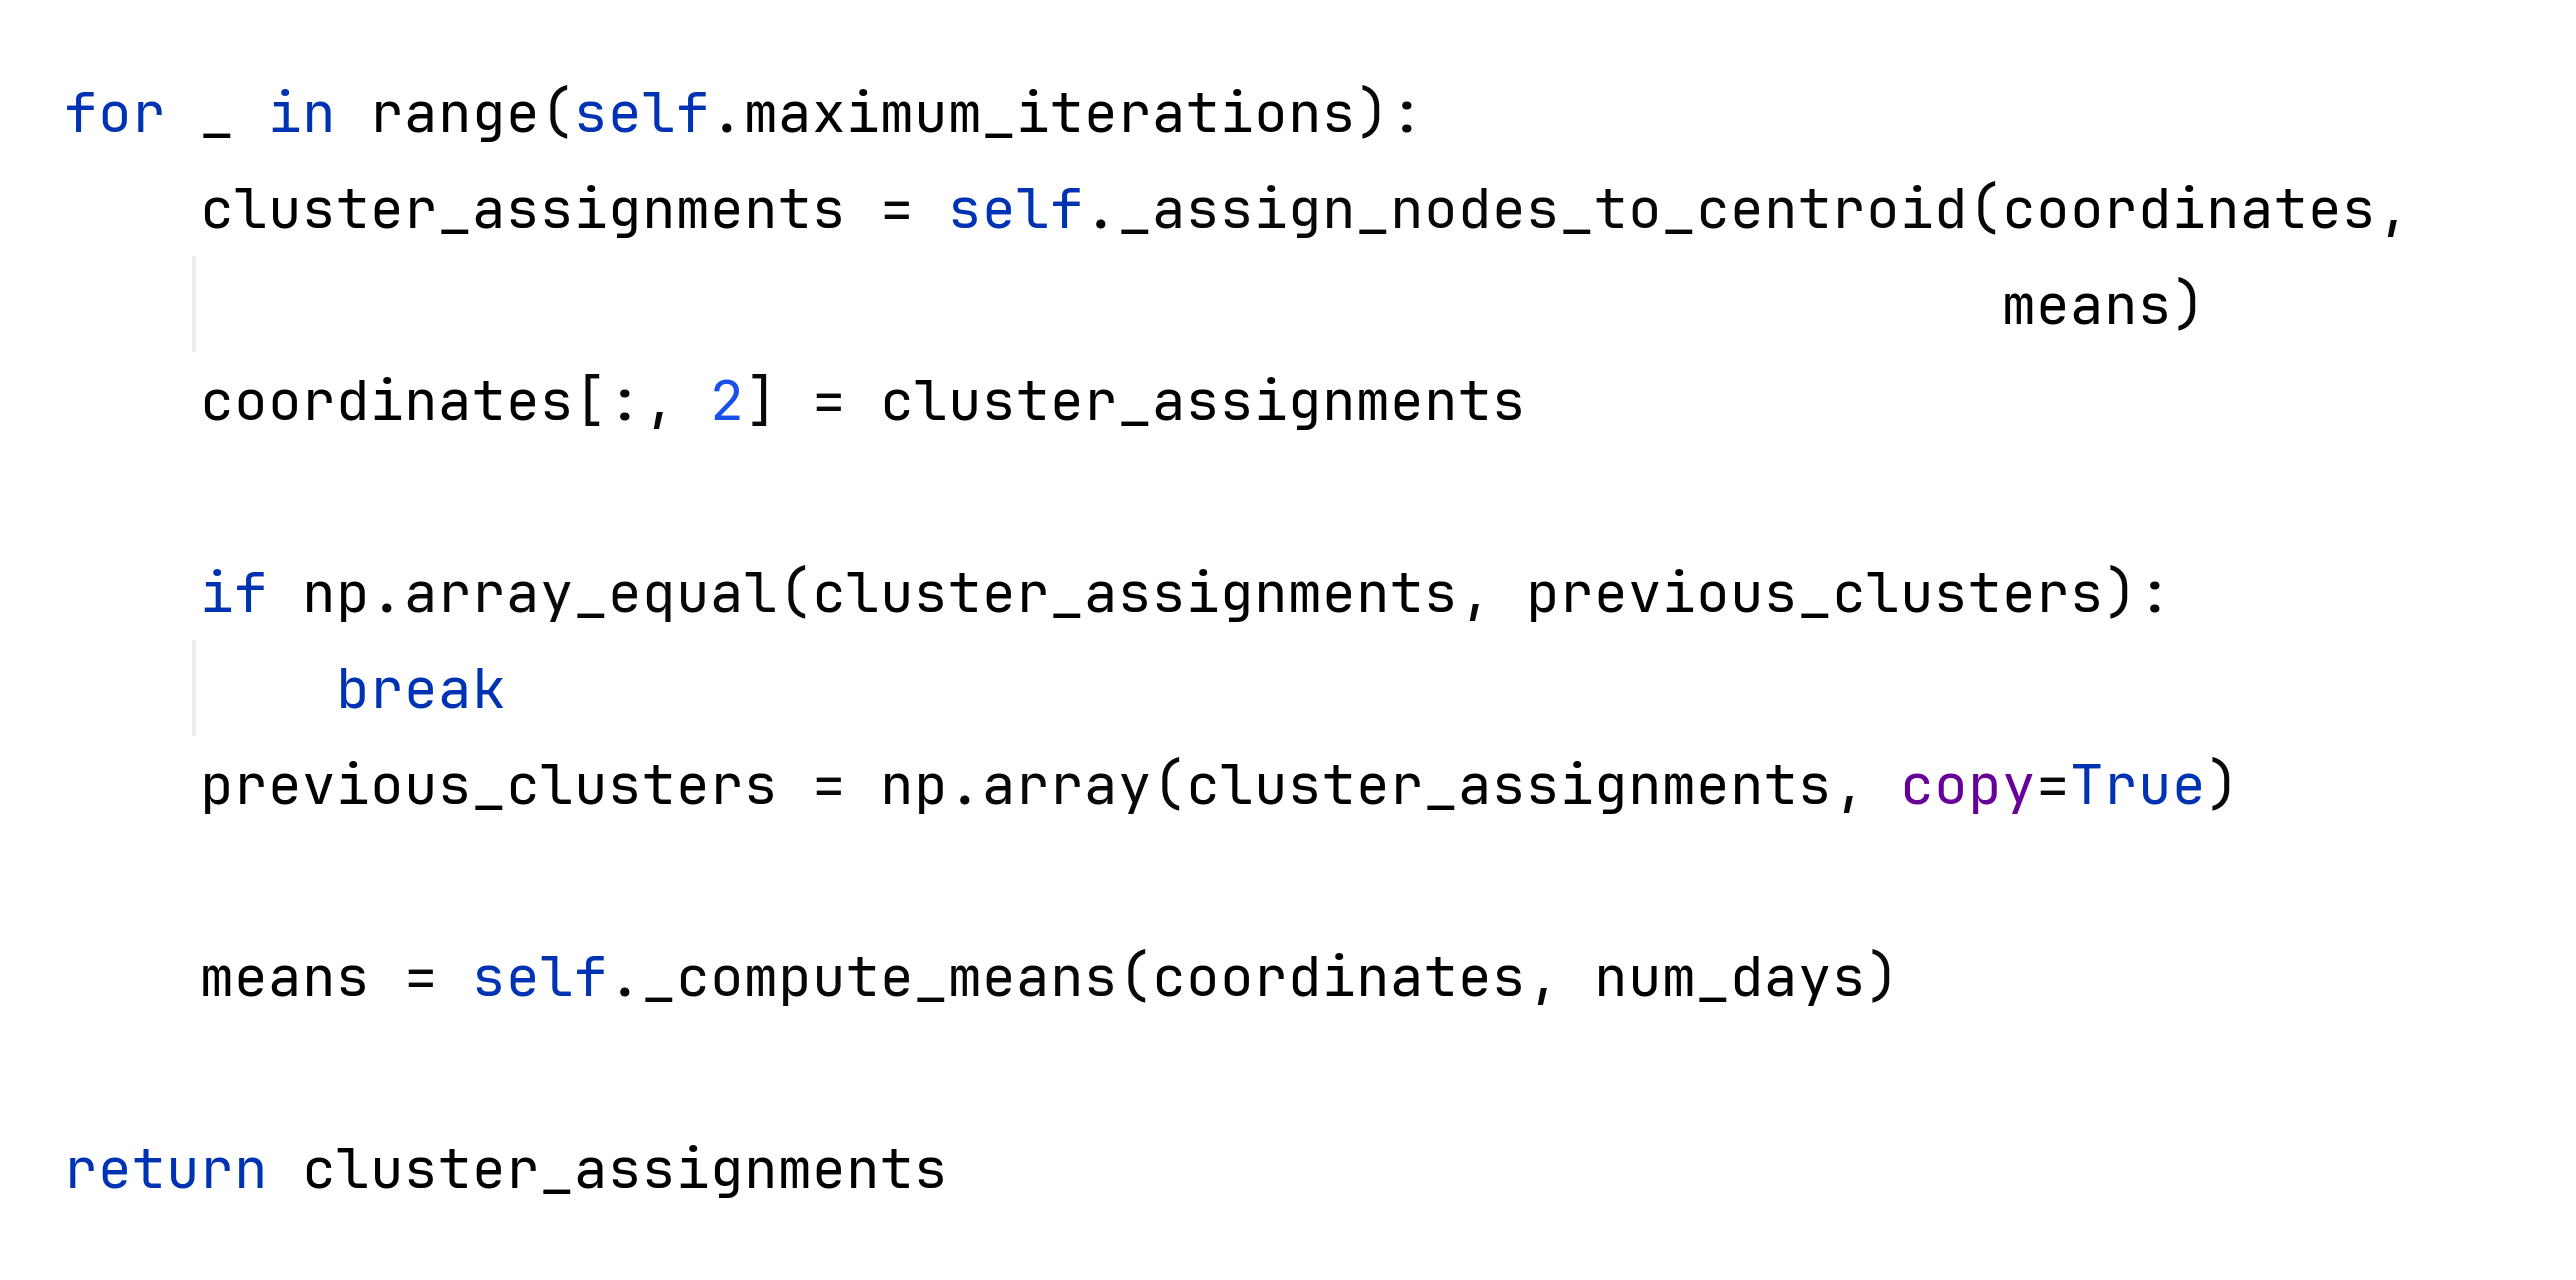
\includegraphics[width = \textwidth]{KMeans.find_clusters}
    \caption{Code from KMeans.find\_clusters in algorithms\textbackslash clustering.py}
    \label{fig:KMeans.find_clusters}
\end{figure}

\noindent
Figure~\ref{fig:KMeans_London_Step1} shows an example of the iterations of a K-Means algorithm run on an input with
12 points of interest around London to be visited over 3 days.
\begin{figure}[H]
    \ContinuedFloat*
    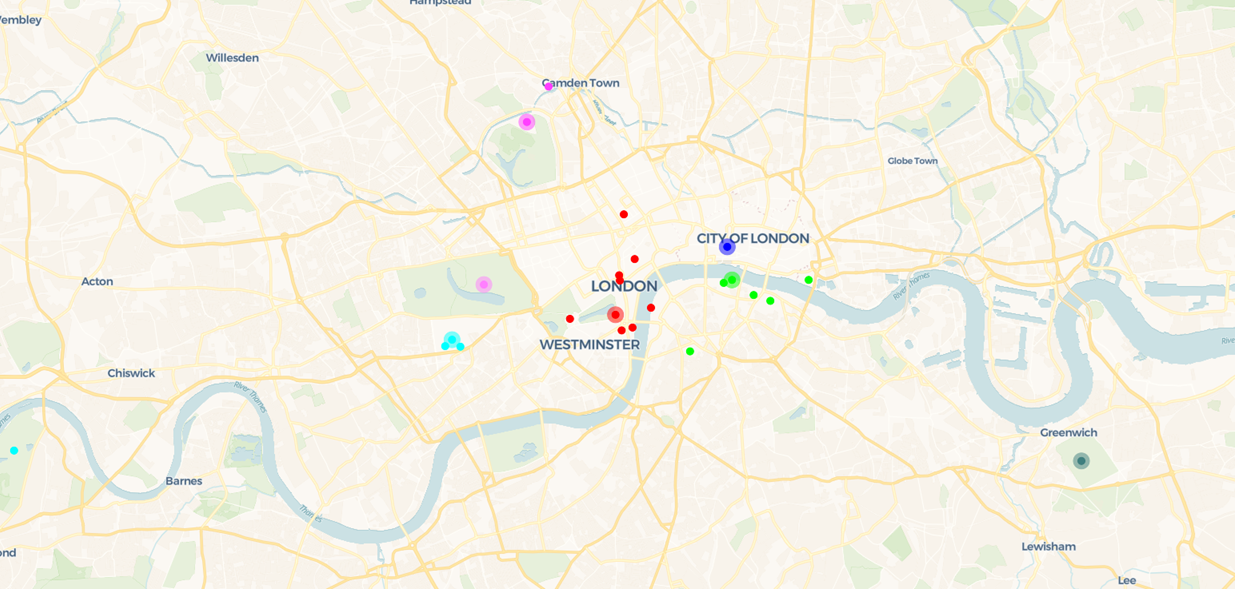
\includegraphics[width = \textwidth]{KMeans_London_Step1}
    \caption{K-Means example Step 1, Initial centroid positions and cluster assignments.}
    \label{fig:KMeans_London_Step1}
\end{figure}
\begin{figure}[H]
    \ContinuedFloat
    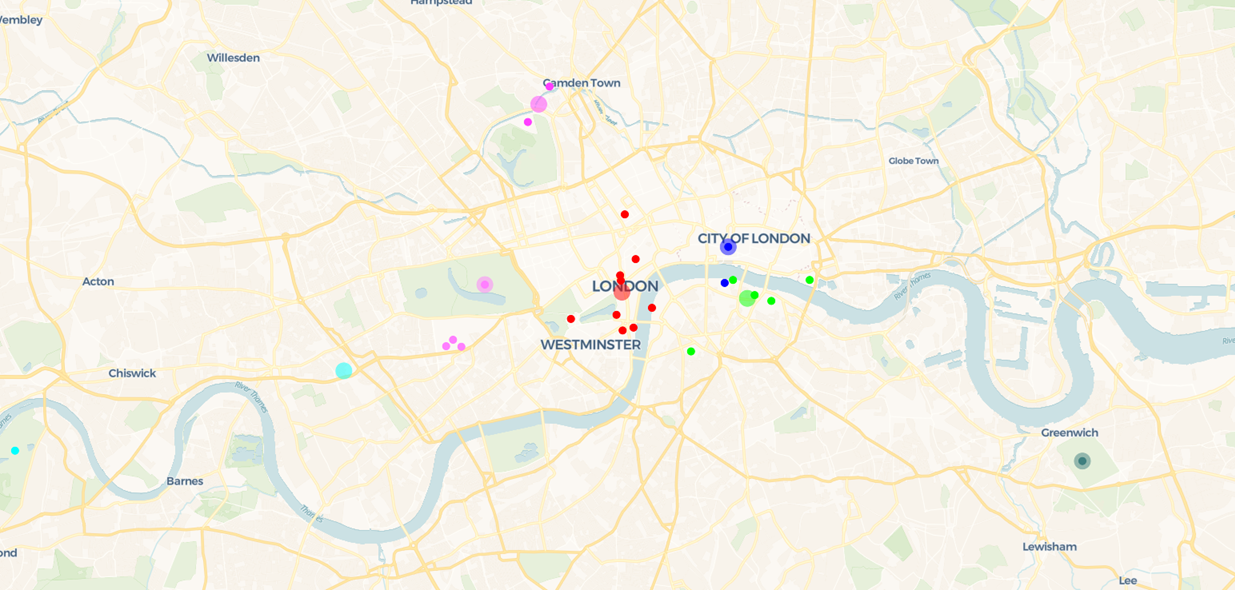
\includegraphics[width = \textwidth]{KMeans_London_Step2}
    \caption{K-Means example Step2, Centroids have been updated, locations are reassigned to their closest centroid.}
    \label{fig:KMeans_London_Step2}
\end{figure}
\begin{figure}[H]
    \ContinuedFloat
    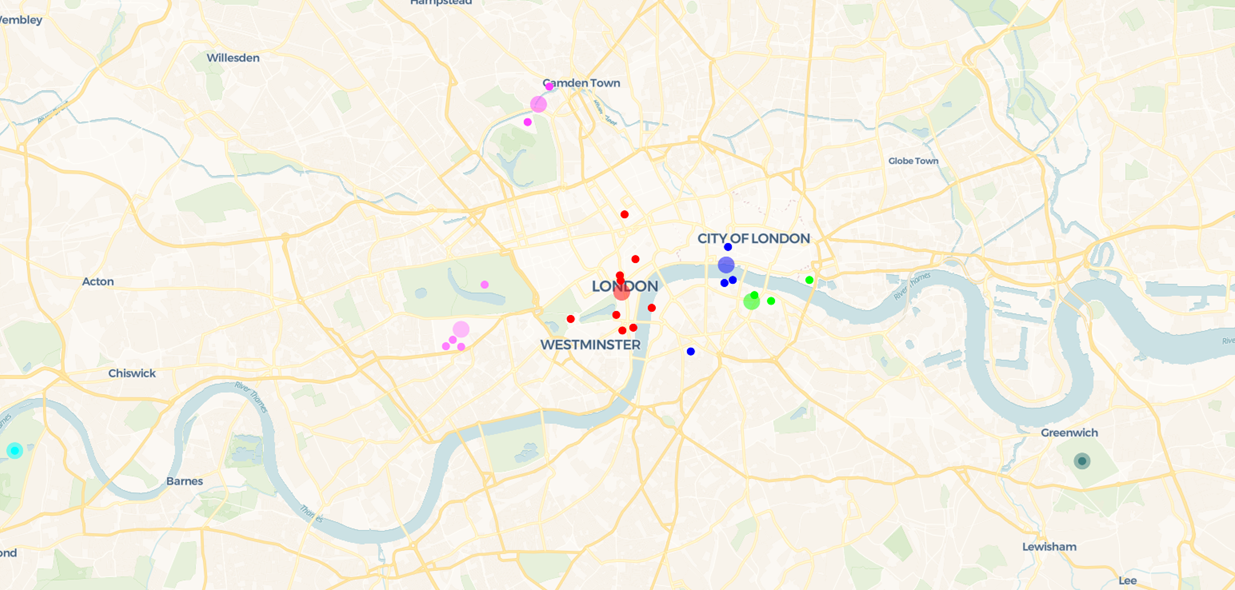
\includegraphics[width = \textwidth]{KMeans_London_Step3}
    \caption{K-Means example Step3, Centroids have updated and no locations have changed cluster, a solution has been found.}
    \label{fig:KMeans_London_Step3}
\end{figure}

\noindent
It is worth noting that K-Means only forms these clusters based on Euclidean distances, grouping together locations
that are close geographically.
However, as formally described in the \hyperref[subsec:objective-function]{Objective Function} section of the
\hyperref[sec:problem-formulation]{Problem Formulation}, a good trip will minimise both the route length of the trip
and the variance between time spent each day.
K-Means does not aim to optimise for the variance between days, it doesn't even consider the time spent at each
location.
Furthermore, while each cluster might be optimised for distance, how close two locations are may not reflect the travel
time between them.
While K-Means does not intentionally optimise for variance between days or consider travel time between locations, it
was still chosen for this project out of curiosity as to how effective a heuristic it might provide.
Hopefully it will offer a simple and computationally efficient baseline for comparison with more complex
algorithms.

\subsubsection{Genetic Clustering}
Genetic clustering applies genetic algorithms to attempt and find the best assignment of locations to clusters.
Genetic algorithms are a type of evolutionary algorithm that aims to mimic biological evolution to find an optimal
solution.
They involve creating a population of potential solutions (individuals) and iteratively improving the population
through selection (keeping the best individuals in the population, akin to natural selection), crossover (combining
individuals to create offspring, akin to sexual reproduction), and mutation (randomly altering the genomes
of individuals in the population, akin to biological mutation).

For us to perform selection, and find the best solutions in a population, we need to assign some fitness to each
individual.
To do this we will combine the cluster assignments with a chosen routing algorithm, and then apply our cost function
to the route found.
This cost will be used to rank our population, helping us find clusters that can produce a good trip.

The performance of Genetic algorithms is highly dependent on its hyperparameters: mutation rate, determining how
common mutation is; crossover rate, determining how often offspring are created via crossover, as opposed to new
additions to the population; population size, determining how many individuals there are per generation; number of
generations, determining how many generations will be evolved to reach a solution; crossover method used,
determining how crossover is performed to create offspring; and in our case, the routing algorithm used, which may
impact how clusters are used to form routes.
These hyperparameters impact both the runtime of the algorithm and the exploration of the search space, indirectly
impacting the quality of the solution.
Genetic clustering has a time complexity of $O(g p r)$, with $g$ being the number of generations, $p$ being the
population size and $r$ being the time complexity of the chosen routing algorithm.\\
\todo{Figure out how to cite time complexity of genetic algorithms. Or go into explanation for our implementation.}

\noindent
For this genetic clustering, an individual is represented by a genome, which will provide a mapping that assigns each
location to a cluster.
Figure~\ref{fig:barcelona-genome-example} shows an example of this.
\begin{figure}[H]
    \centering
    Genome: [0, 0, 0, 1, 1, 1, 2, 2, 2]\\
    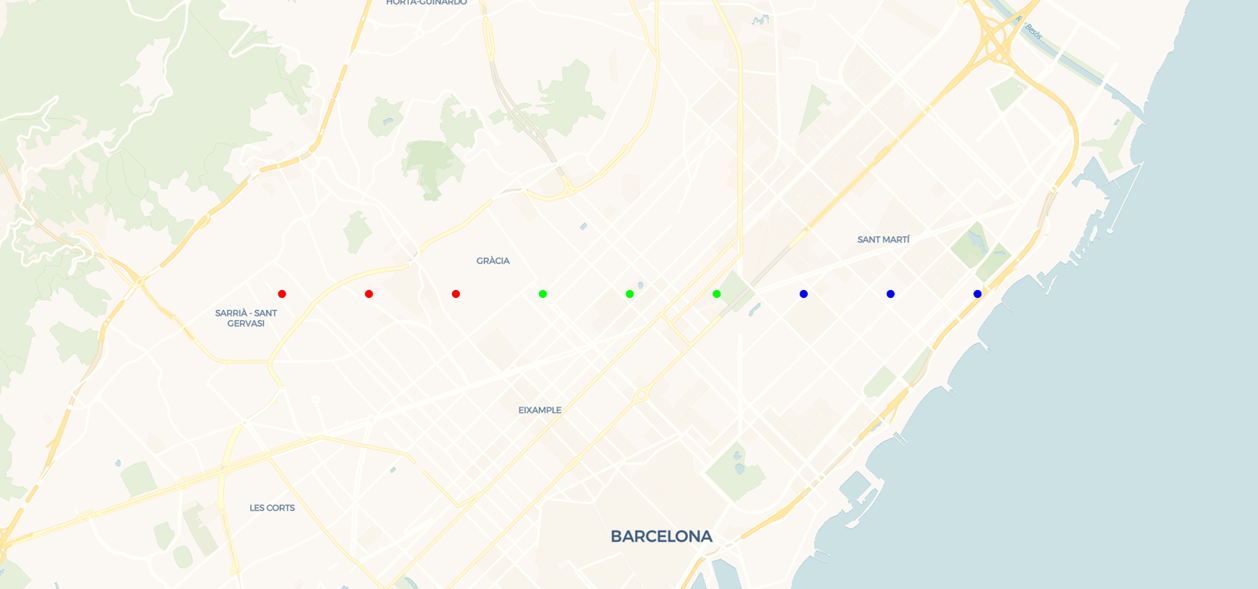
\includegraphics[width = \textwidth]{Barcelona_Genome_Example}
    \caption{Example of how an individual's genome corresponds to cluster assignments.}
    \label{fig:barcelona-genome-example}
\end{figure}

\noindent
These genomes are our target for performing crossover and mutations.
We begin our evolution process by randomly generating an initial population of individuals.
From there, we repeat the following steps until we reach a maximum number of generations:
\begin{enumerate}
    \item Evaluate the fitness of each individual in the population.
    \item Select the best individuals from the population, these will be carried over into the next generation, as
    well as be used to create offspring.
    \item Generate new population using crossover and mutation.
\end{enumerate}

\noindent
As previously discussed, we will evaluate the fitness of each individual by applying a routing algorithms to the
clusters defined by the genome, and then applying our cost function to the resulting route.
Figure~\ref{fig:GeneticClustering._evaluate_population} shows this route finding and evaluation.
\begin{figure}[H]
    \centering
    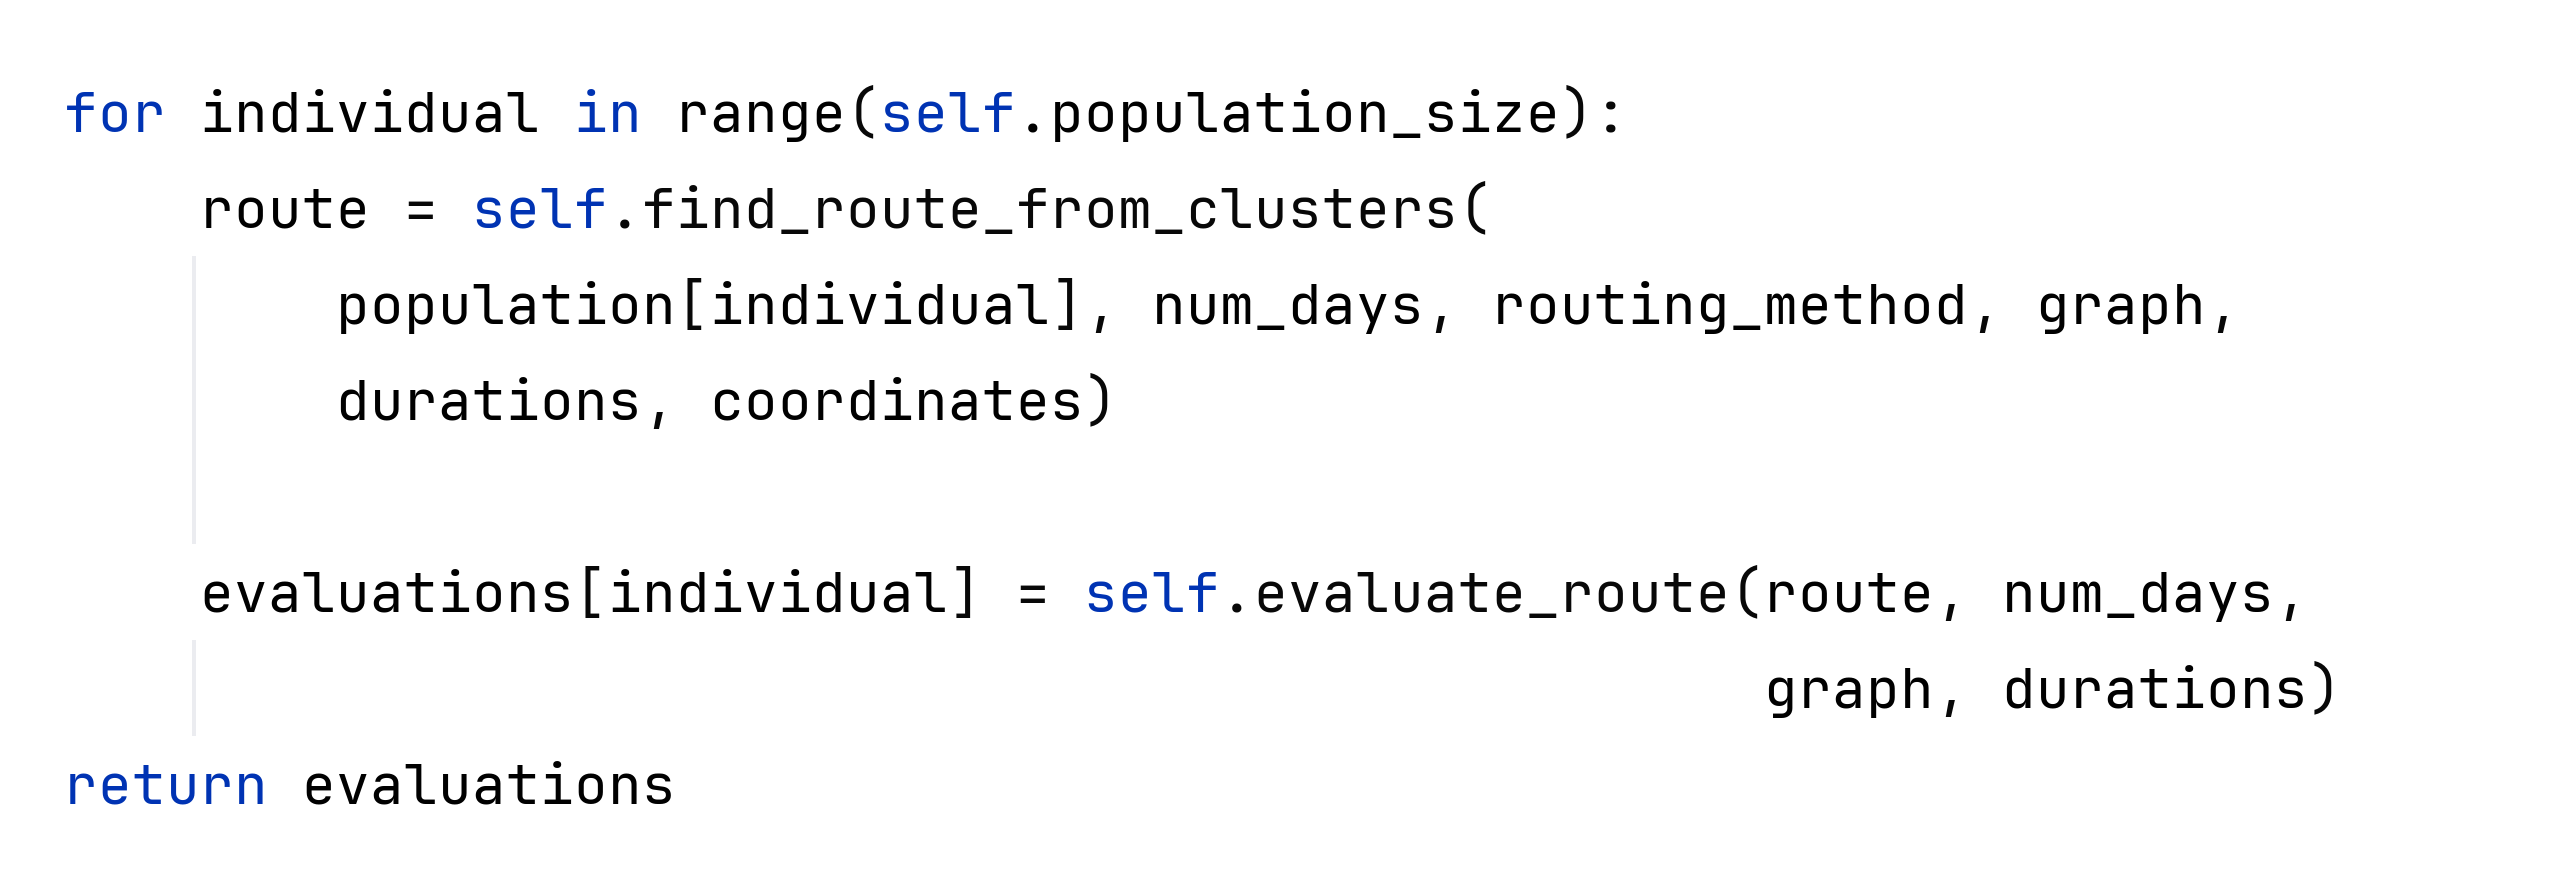
\includegraphics[width = \textwidth]{GeneticClustering._evaluate_population}
    \caption{Code from GeneticClustering.\_evaluate\_population in algorithms\textbackslash clustering.py}
    \label{fig:GeneticClustering._evaluate_population}
\end{figure}

\noindent
The methods called in figure~\ref{fig:GeneticClustering._evaluate_population} are those previously shown in
figure~\ref{fig:Clustering.find_route_from_clusters} (find\_route\_from\_clusters) and
figure~\ref{fig:Algorithm.evaluate_route} (evaluate\_route).
Once the population has been evaluated, the best two individuals are chosen as parents, as figure~\ref{fig:GeneticClustering.find_clusters.select_parents}
shows.
\begin{figure}[H]
    \centering
    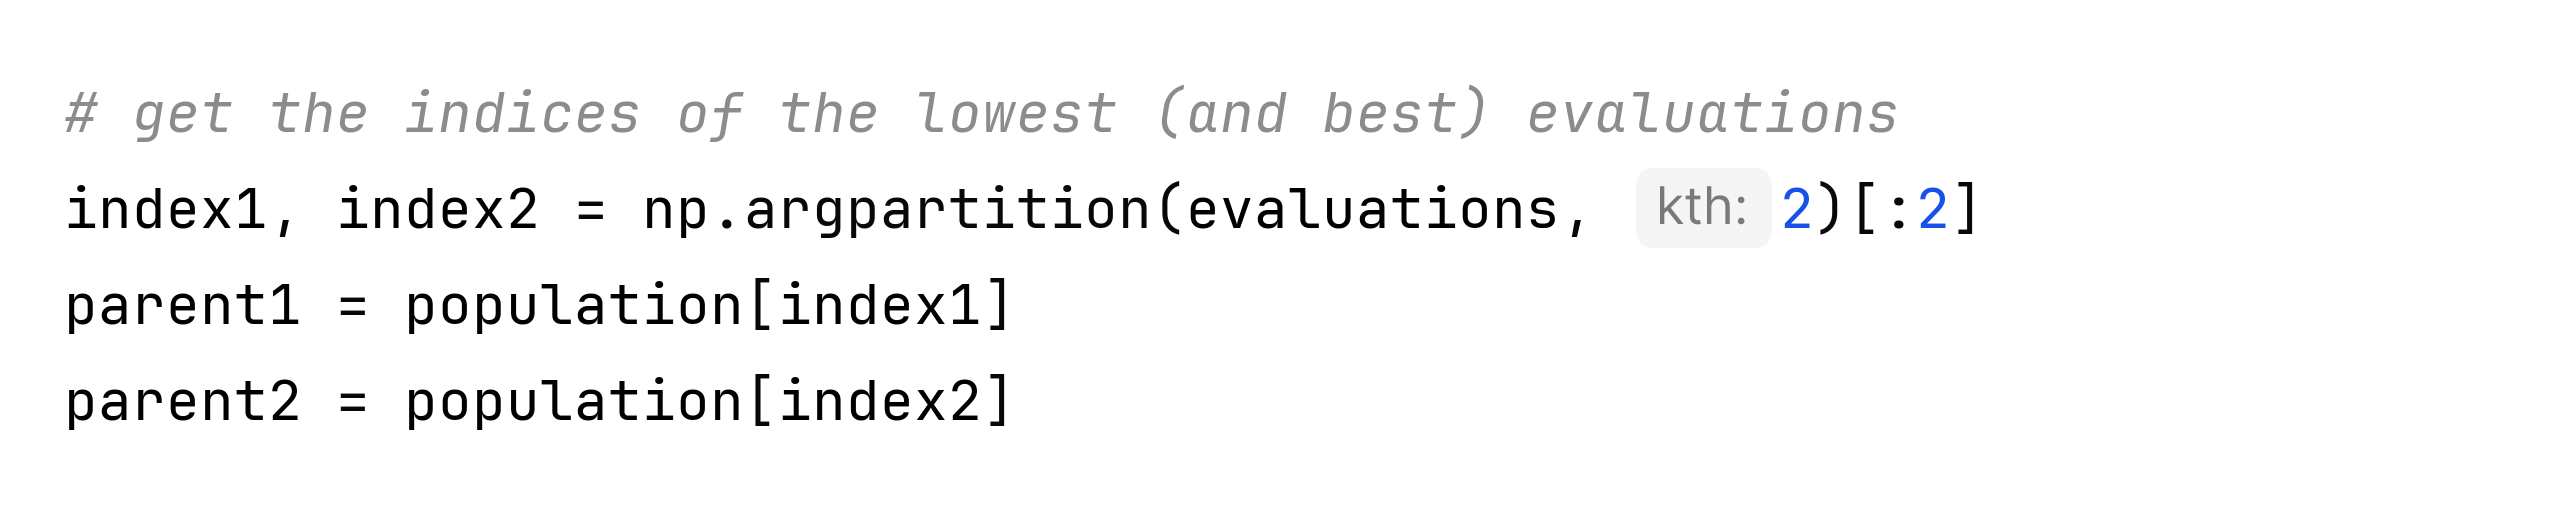
\includegraphics[width = \textwidth]{GeneticClustering.find_clusters.select_parents}
    \caption{Code from GeneticClustering.find\_clusters in algorithms\textbackslash clustering.py}
    \label{fig:GeneticClustering.find_clusters.select_parents}
\end{figure}

\noindent
Excluding the two parents, who will be copied over, the next generation will be created via crossover and mutation,
or through random generation.
We include some randomly generated individuals in an effort to increase genetic diversity and exploration of the
search space.
Figure ~\ref{fig:GeneticClustering.find_clusters.crossover} shows how this is decided in our implementation.
For each individual a random number is generated between 0 and 1, if this number is lower than our crossover rate
the individual is created via crossover, otherwise it will be randomly generated.
\begin{figure}[H]
    \centering
    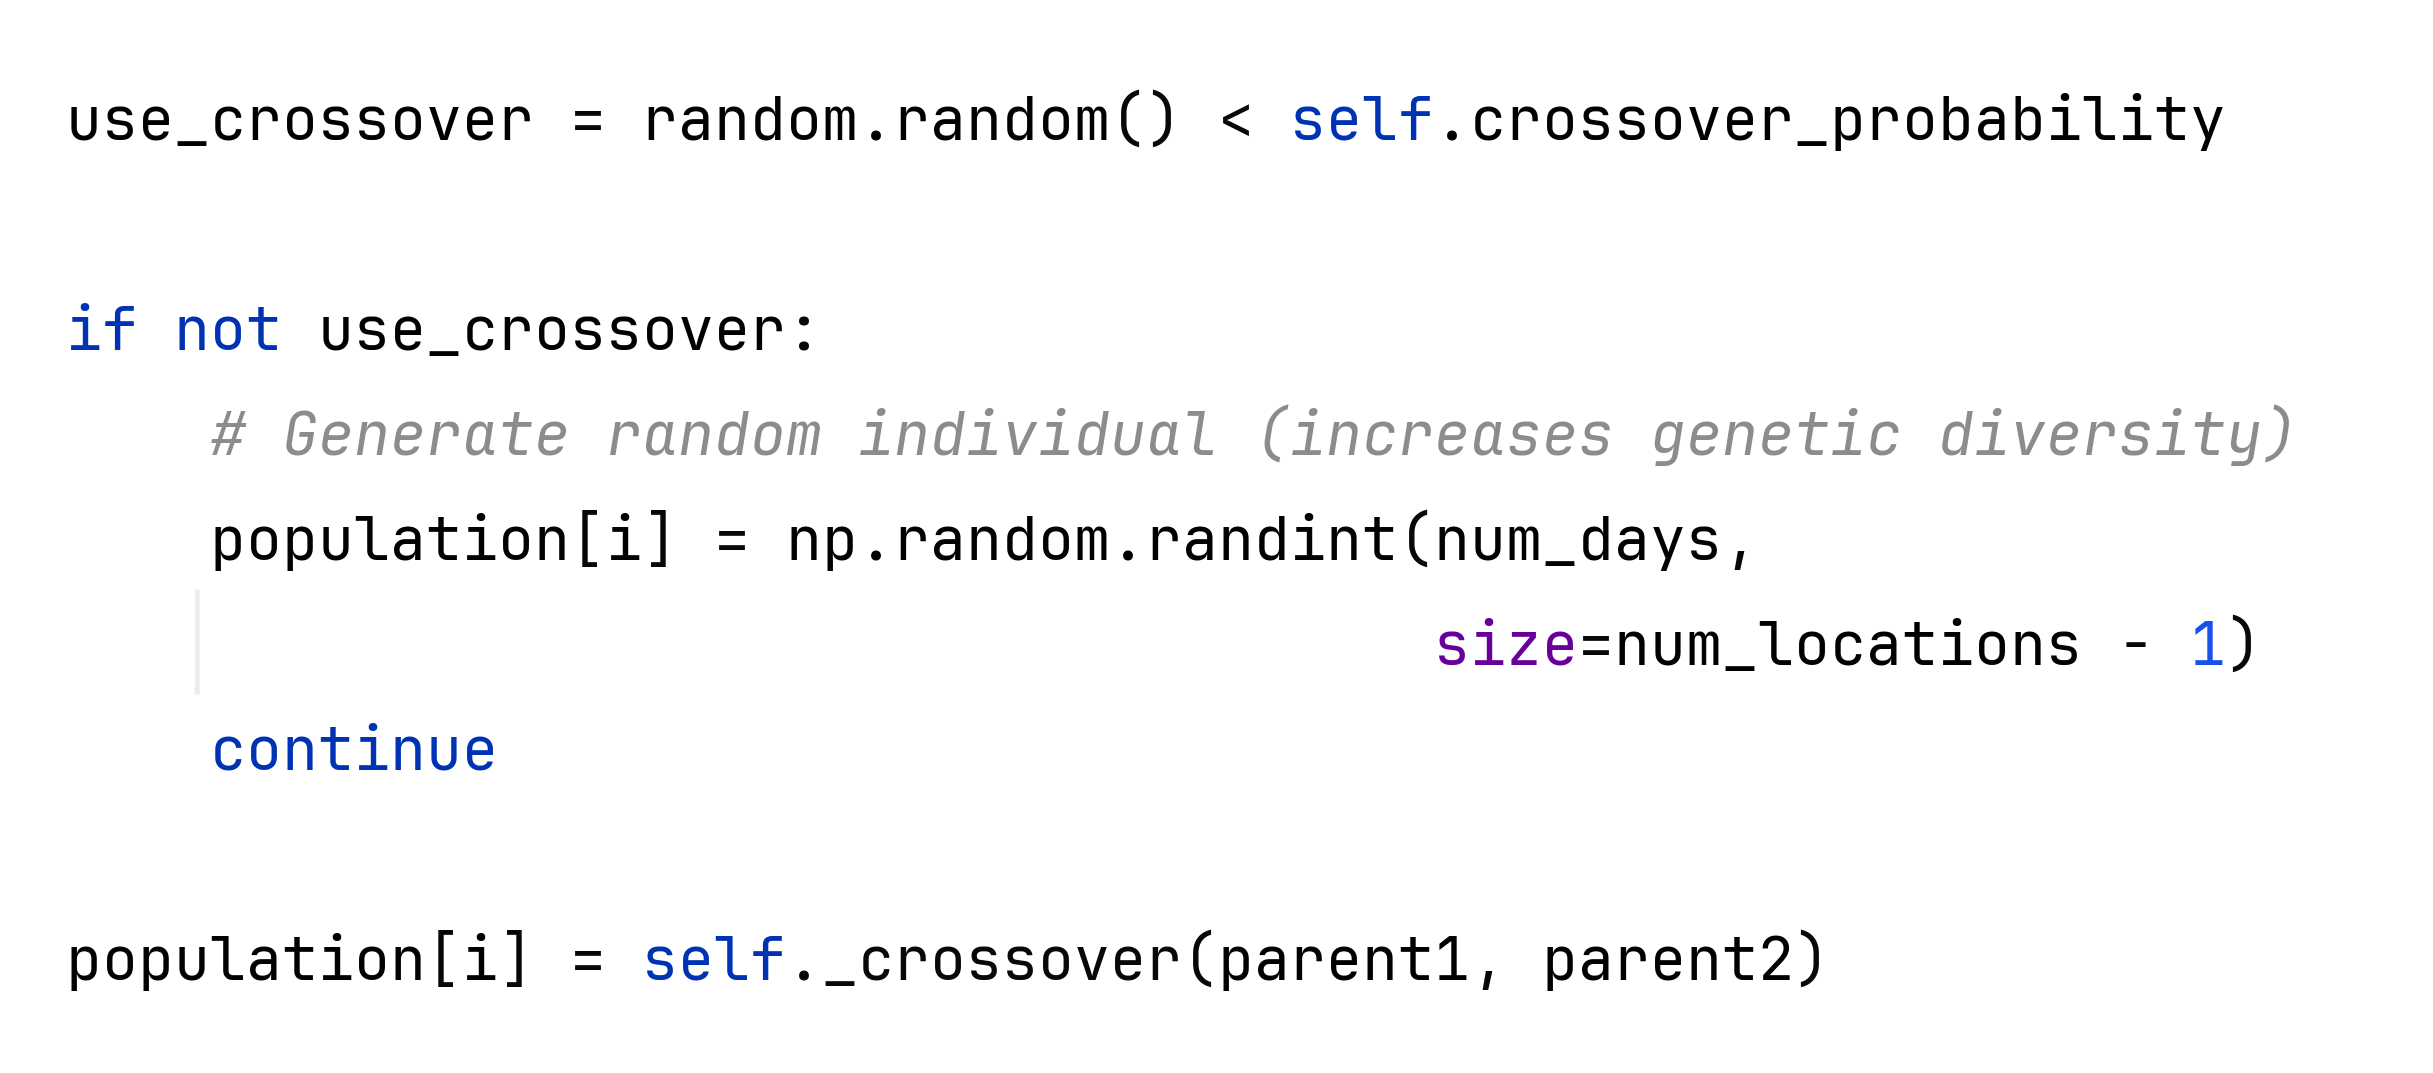
\includegraphics[width = \textwidth]{GeneticClustering.find_clusters.crossover}
    \caption{Code from GeneticClustering.find\_clusters in algorithms\textbackslash clustering.py}
    \label{fig:GeneticClustering.find_clusters.crossover}
\end{figure}

\noindent
For our implementation of crossover, we will be performing a uniform crossover, using crossover masks.
A crossover mask is a bit array the same length as the genome, with the parity of each bit indicating which parent
to choose from for the corresponding bit in the created genome.
In a uniform crossover mask, each bit has an 50\% chance of being a 0 or 1, meaning that each bit in the offspring
genome has an equal chance of being from either parent
\todo{Cite Uniform Crossover in Genetic Algorithms, Giblert Syswerda.}.
If the two parents, being the best individuals in a population, agree on a bit it then it would appear likely it's a
good choice.
With our implementation of crossover, the offspring will always copy over the bits that parents agree on.
Figure~\ref{fig:Crossover_Mask_Example} shows an example of how a crossover mask can be used to create a child from
two parents, the example uses a hypothetical input including 6 locations and 3 clusters.
\begin{figure}[H]
    \centering
    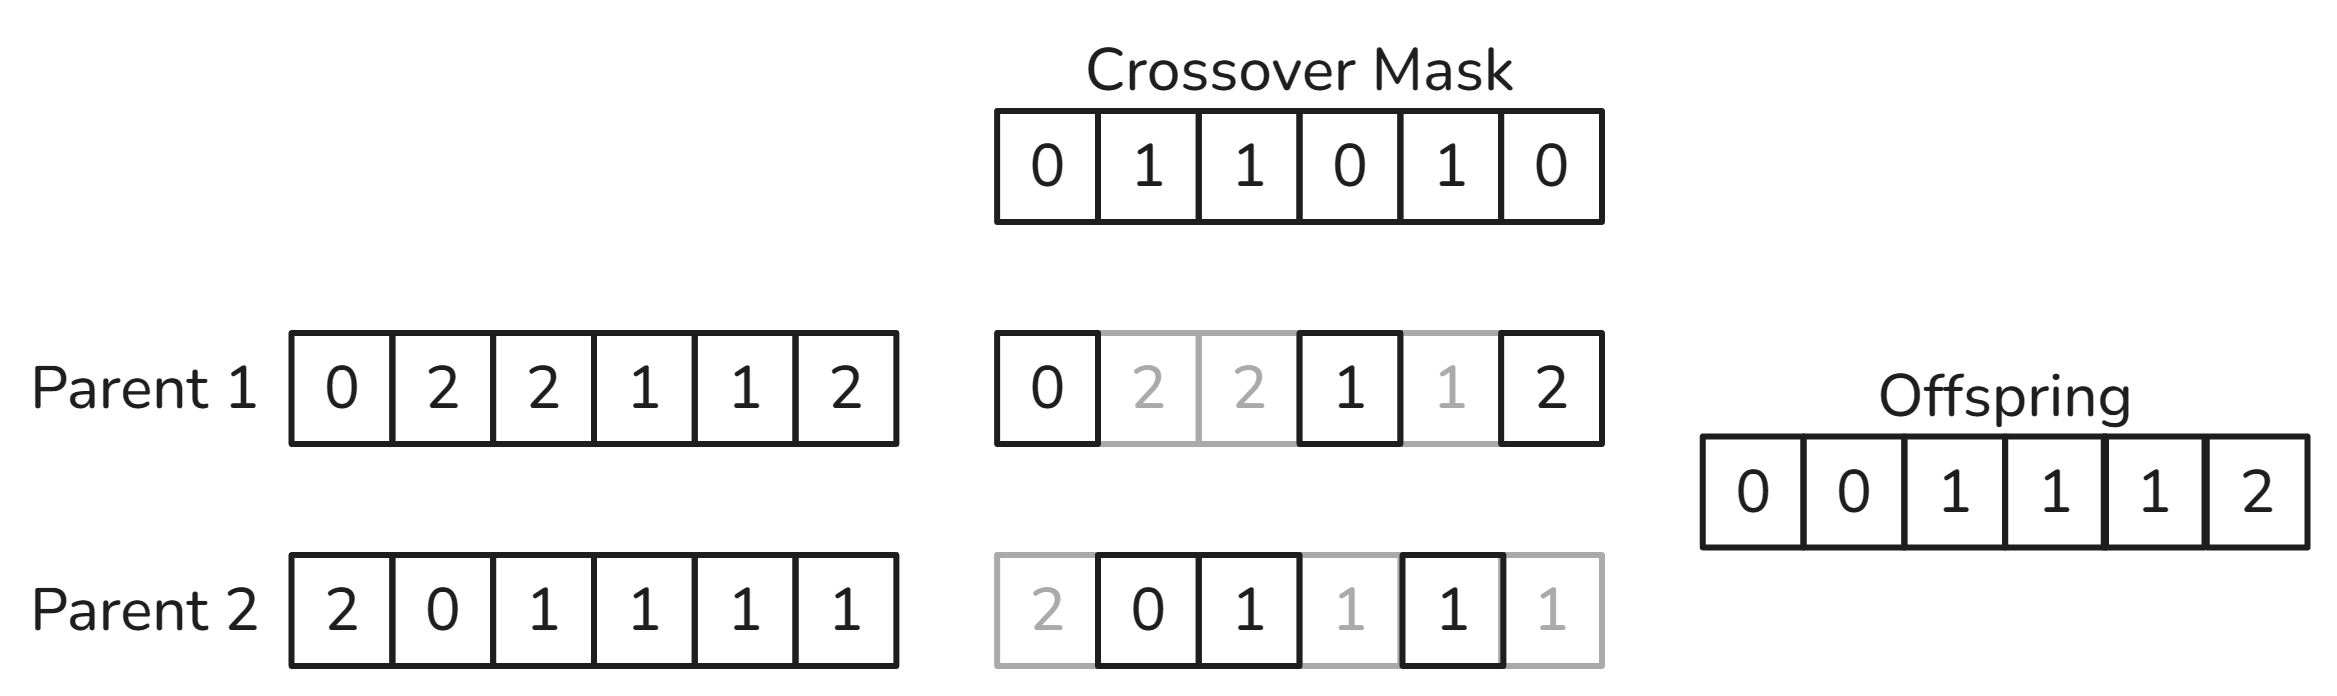
\includegraphics[width = \textwidth]{Crossover_Mask_Example}
    \caption{Example of using a crossover mask to create a child from two parents.}
    \label{fig:Crossover_Mask_Example}
\end{figure}

\noindent
There is however, one slight issue with applying this method to our problem.
In the example shown in figure~\ref{fig:Crossover_Mask_Example}, parent 1's 0th cluster only includes the first
location, similarly, parent 2's 2nd cluster also only includes the first location.
Both parents are forming a cluster using these locations, however due to them being labelled differently, the
offspring produced did not continue this clustering.
To solve this problem a genome's clusters will be relabelled in order of their appearance in the genome, ensuring
consistency between parents.
Figure~\ref{fig:Crossover_Mask_Relabelling_Example} shows an example of this applied to the parents in figure~\ref{fig:Crossover_Mask_Example},
and figure~\ref{fig:GeneticClustering._relabel_individuals_clusters} shows how this is accomplished in our python
implementation.
\begin{figure}[H]
    \centering
    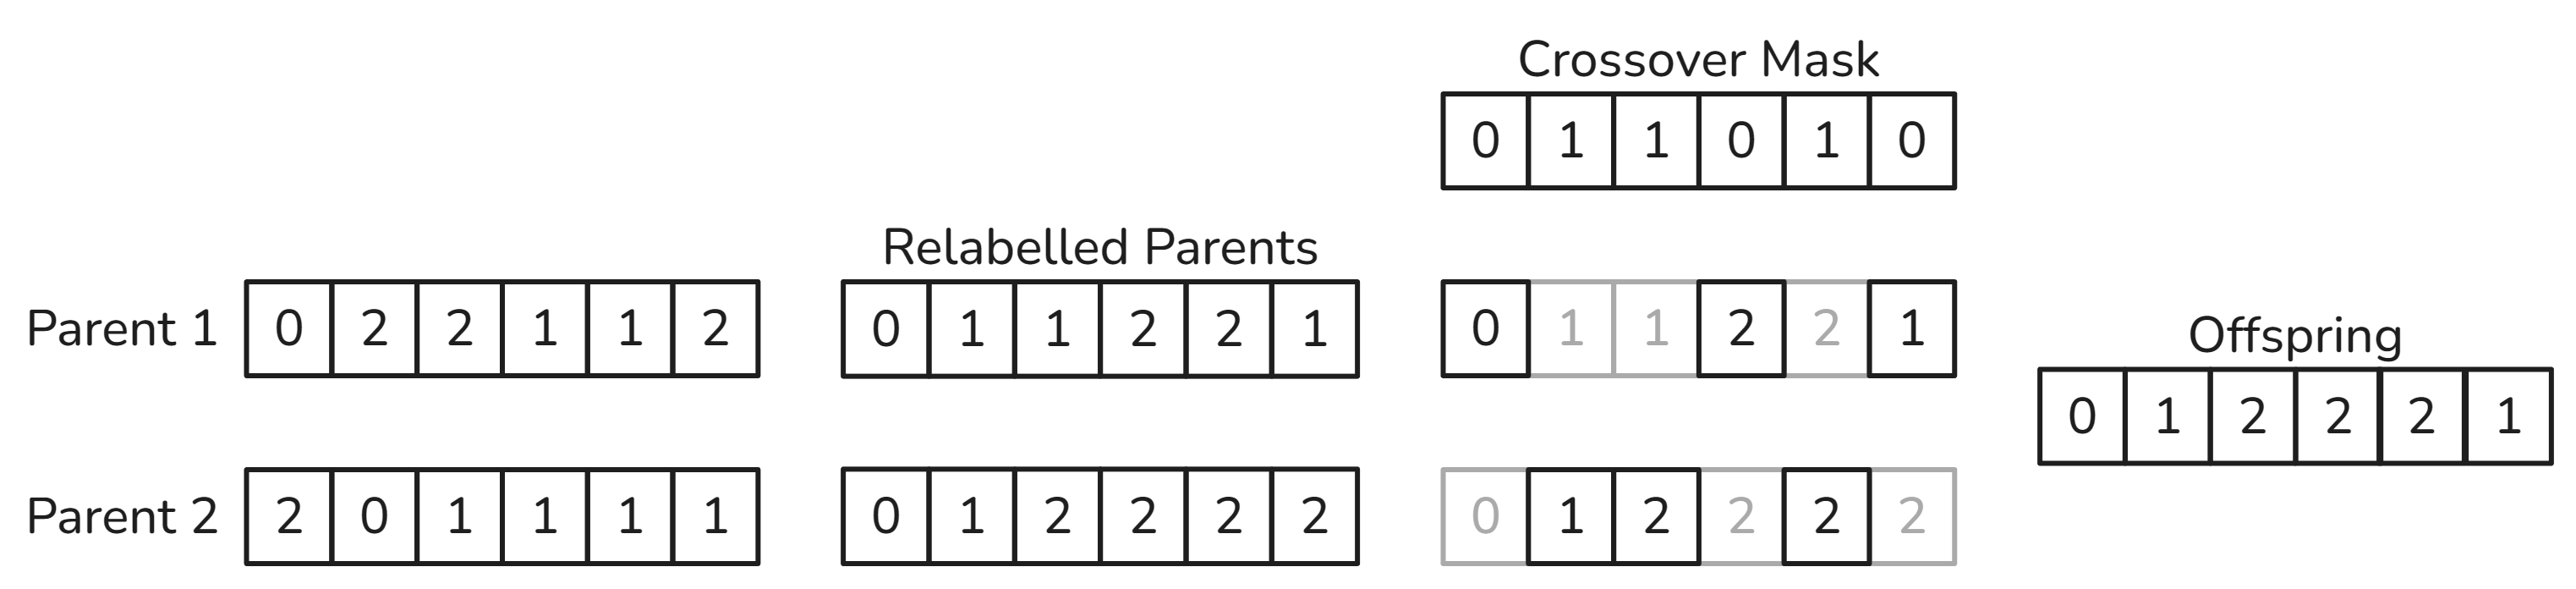
\includegraphics[width = \textwidth]{Crossover_Mask_Relabelling_Example}
    \caption{Example of relabelling a parent's clusters and the resultant offspring}
    \label{fig:Crossover_Mask_Relabelling_Example}
\end{figure}
\begin{figure}[H]
    \centering
    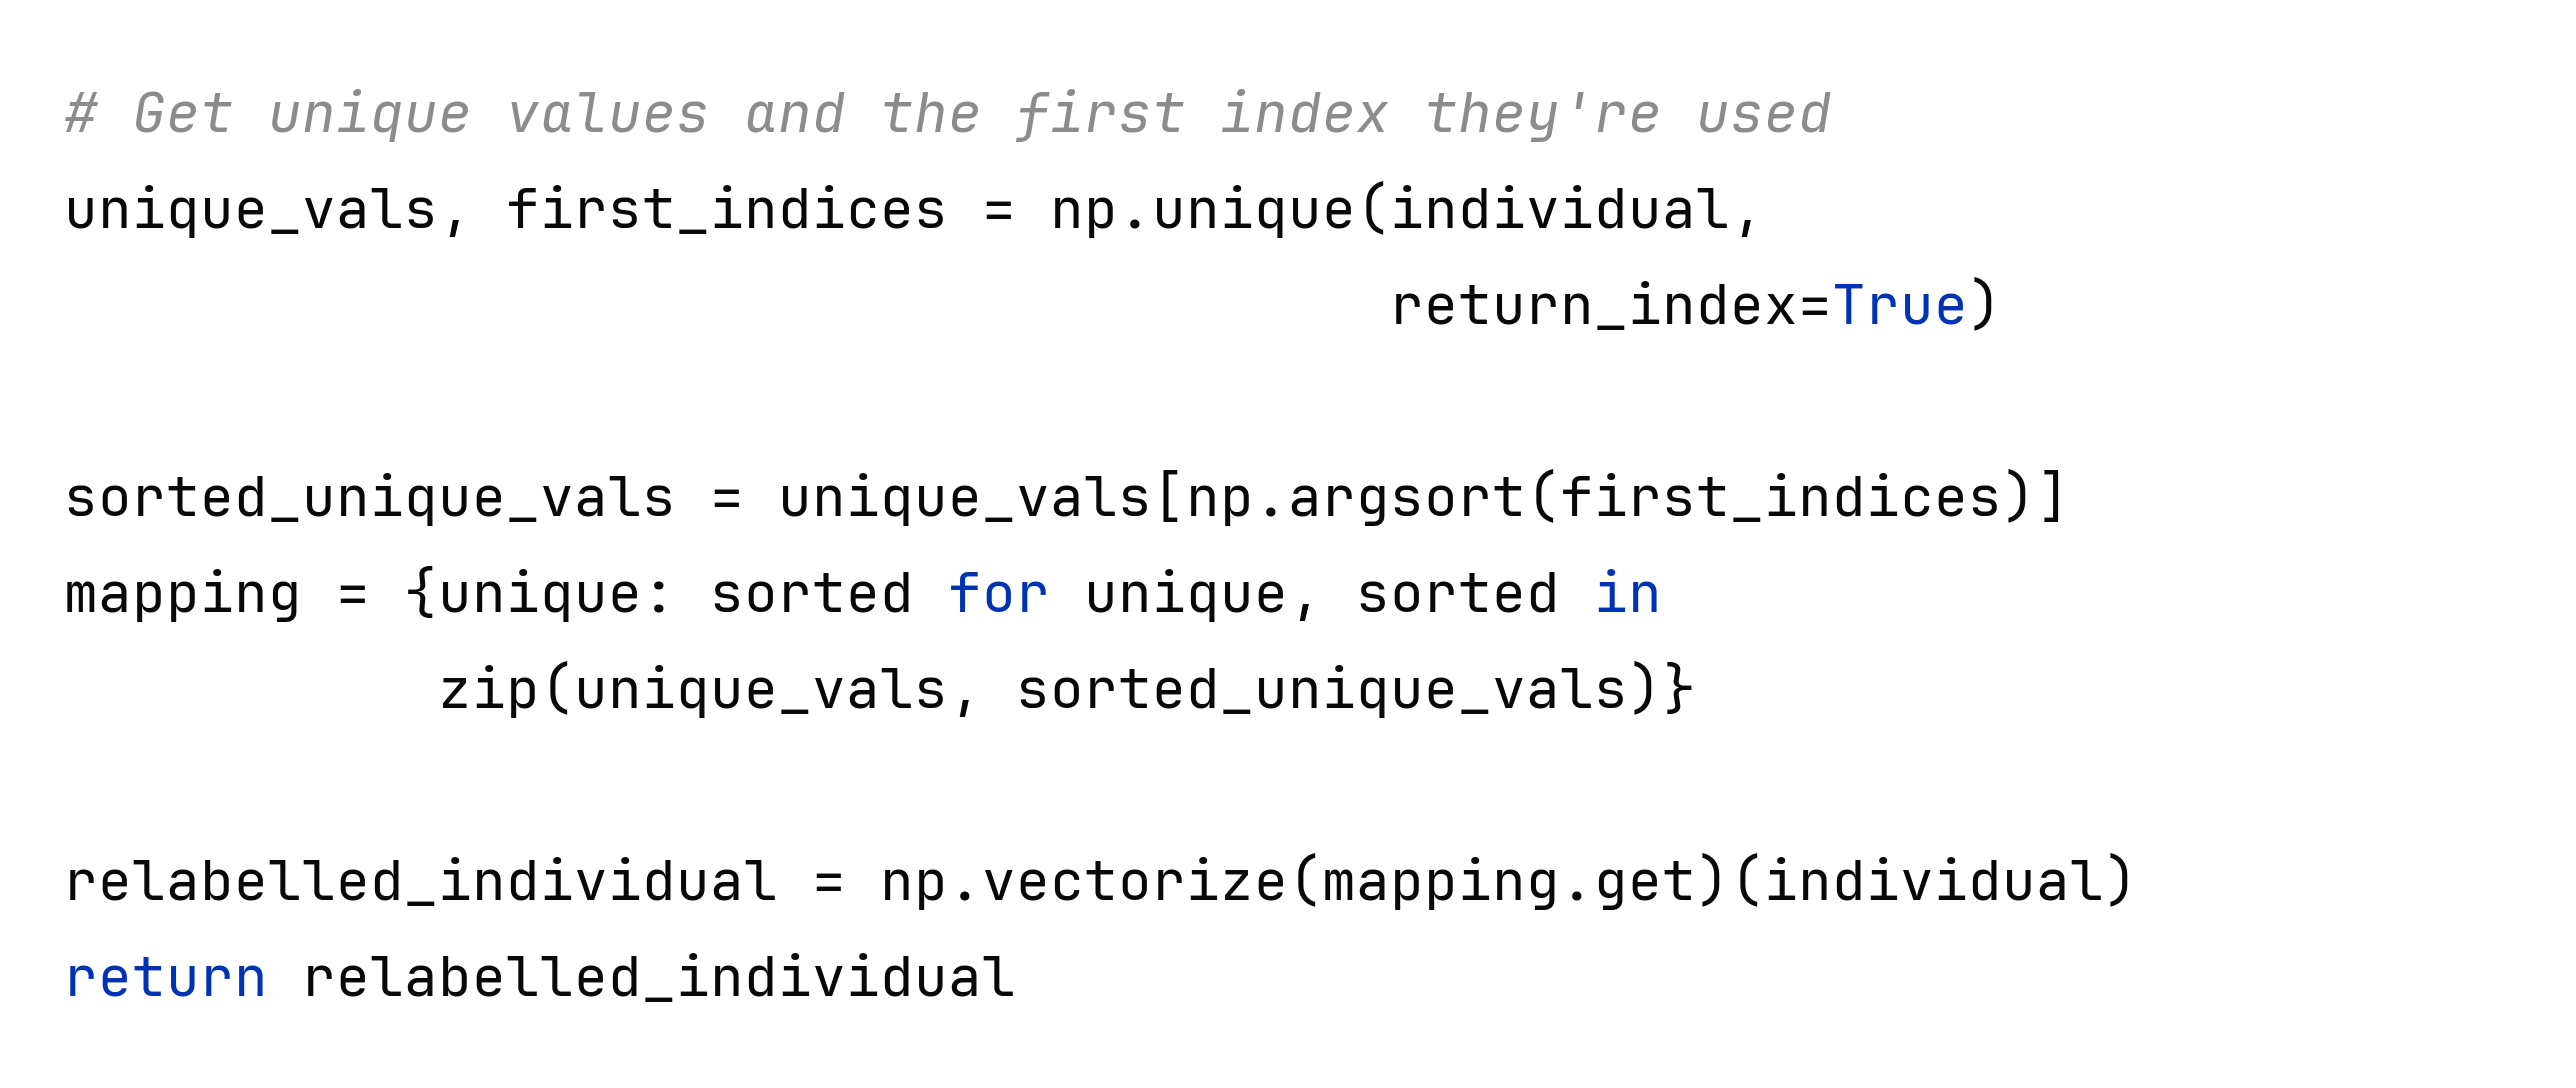
\includegraphics[width = \textwidth]{GeneticClustering._relabel_individuals_clusters}
    \caption{Code from GeneticClustering.\_relabel\_individuals\_clusters in algorithms\textbackslash clusterin.py}
    \label{fig:GeneticClustering._relabel_individuals_clusters}
\end{figure}

\noindent
After this relabelling, crossover can be performed without issue.
Figure~\ref{fig:GeneticClustering._crossover} shows our python implementation of this.
\begin{figure}[H]
    \centering
    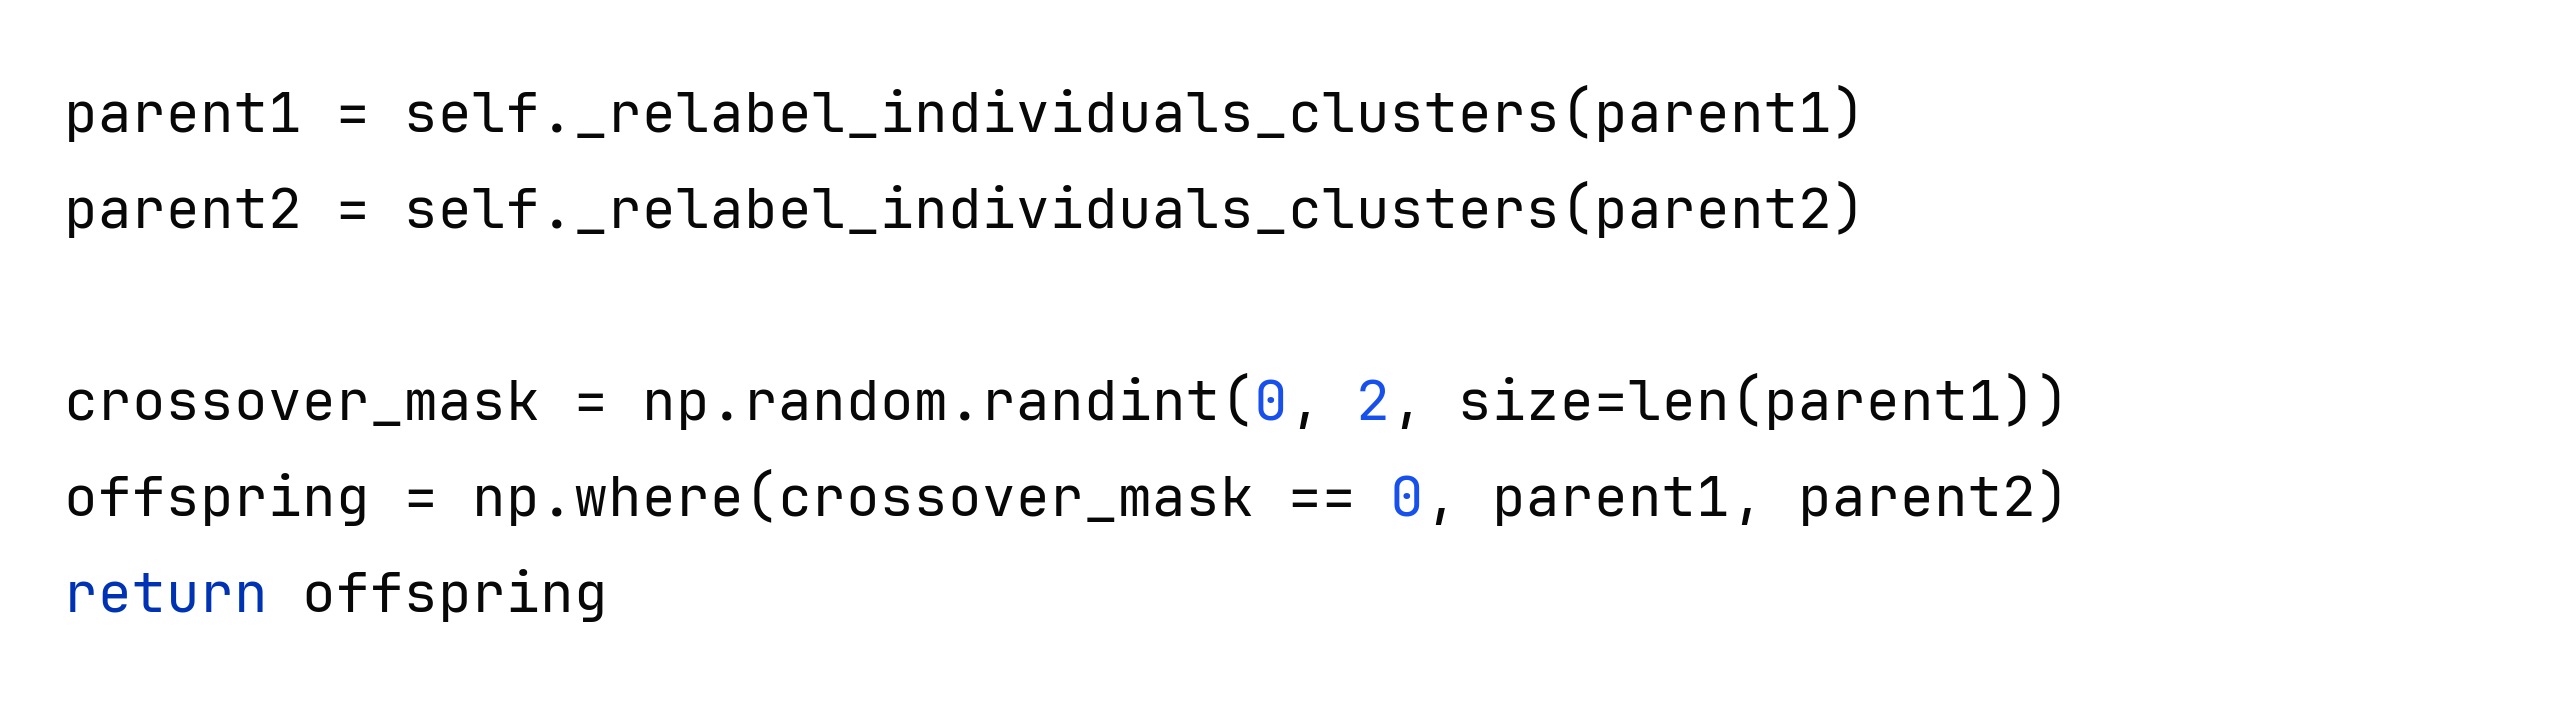
\includegraphics[width = \textwidth]{GeneticClustering._crossover}
    \caption{Code from GeneticClustering.\_crossover in algorithms\textbackslash clustering.py}
    \label{fig:GeneticClustering._crossover}
\end{figure}

After crossover is complete, we randomly mutate the created offspring in the hopes of increasing genetic diversity
and escaping local optima.
We mutate our genome by iterating through each gene and randomly deciding if it will mutate or not, the likeliness
of mutation is decided by our mutation rate.
If a gene is chosen to mutate, it will assign itself to a random cluster.
Figure~\ref{fig:GeneticClustering.find_clusters.mutation} shows how this is implemented in python.
\begin{figure}[H]
    \centering
    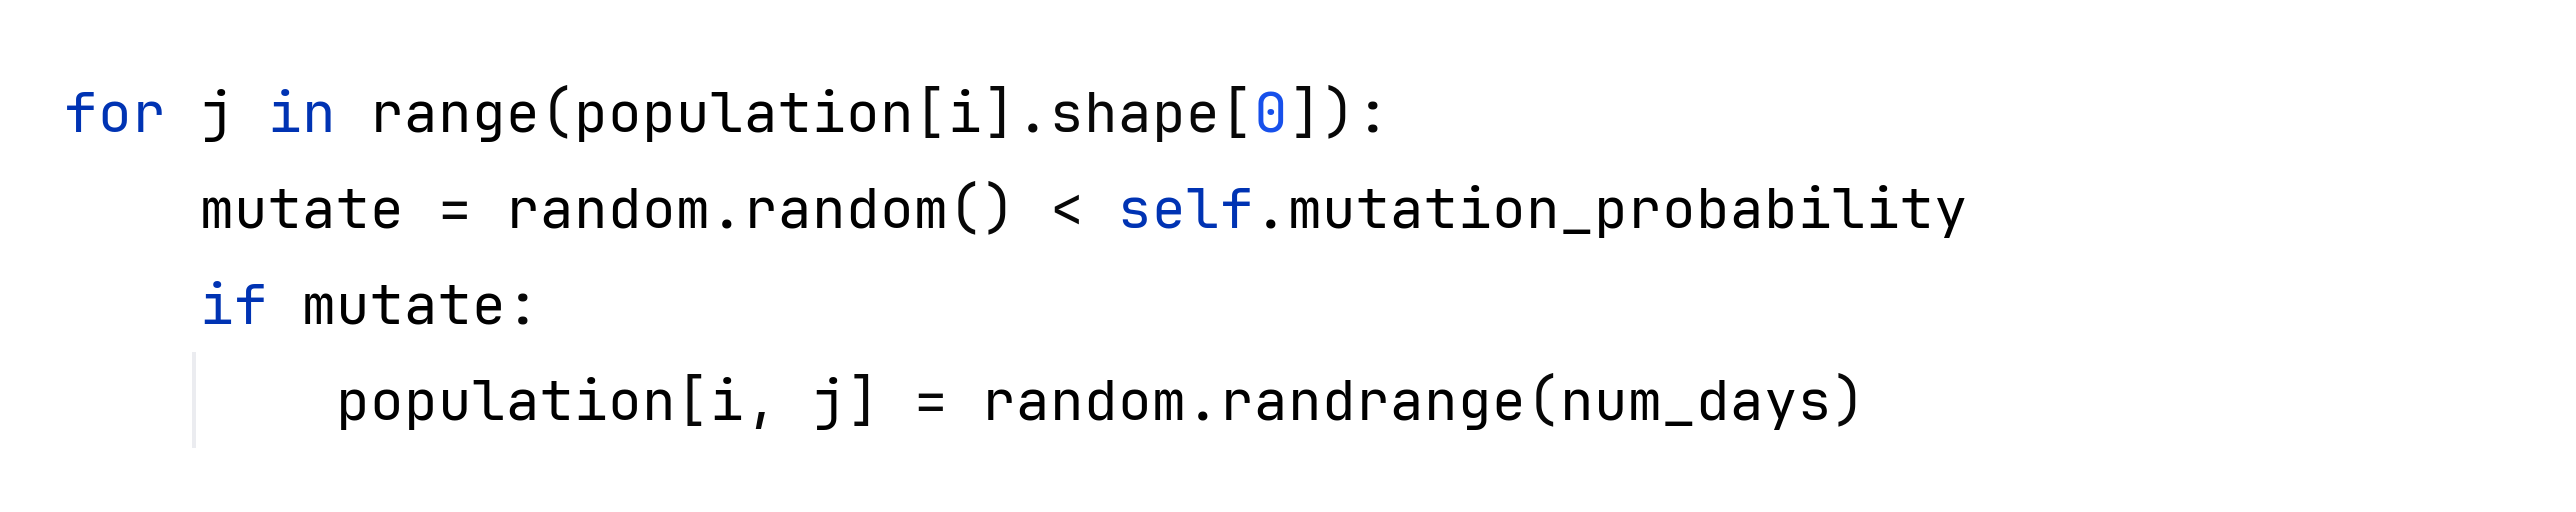
\includegraphics[width = \textwidth]{GeneticClustering.find_clusters.mutation}
    \caption{Code from GeneticClustering.find\_clusters in algorithms\textbackslash clustering.py}
    \label{fig:GeneticClustering.find_clusters.mutation}
\end{figure}

\noindent
After the new population has been created, we restart the process for the next generation, repeating these steps
until a maximum number of generations is reached.
By time evolution is complete the population will hopefully have converged on a good solution.
Figure~\ref{fig:GeneticClustering_London_Generation1} shows an example of genetic clustering using the same input as for the
K-Means example in figure~\ref{fig:KMeans_London_Step1}.
In the example, genetic clustering is used alongside greedy routing (to be covered in section~\ref{subsubsec:greedy-routing})
to form a complete trip, the best routes found within their respective generations are shown.
The genetic clustering was run for 30 generations with a population size of 12, a crossover rate of 0.9 was used
alongside a mutation rate of 0.1.
Figure~\ref{fig:GeneticClustering_London_Evaluations} shows a line graph of the best evaluation found for each
generation.
\begin{figure}[H]
    \ContinuedFloat*
    \centering
    \includegraphics[width = \textwidth]{GeneticClustering_London_Generation1}
    \caption{Genetic Clustering example, best route found in Generation 1.}
    \label{fig:GeneticClustering_London_Generation1}
\end{figure}
\begin{figure}[H]
    \ContinuedFloat
    \centering
    \includegraphics[width = \textwidth]{GeneticClustering_London_Generation5}
    \caption{Genetic Clustering example, best route found in Generation 5.}
    \label{fig:GeneticClustering_London_Generation2}
\end{figure}
\begin{figure}[H]
    \ContinuedFloat
    \centering
    \includegraphics[width = \textwidth]{GeneticClustering_London_Generation10}
    \caption{Genetic Clustering example, best route found in Generation 10.}
    \label{fig:GeneticClustering_London_Generation10}
\end{figure}
\begin{figure}[H]
    \ContinuedFloat
    \centering
    \includegraphics[width = \textwidth]{GeneticClustering_London_Generation30}
    \caption{Genetic Clustering example, best route found in Generation 30, evolution is now complete.}
    \label{fig:GeneticClustering_London_Generation30}
\end{figure}
\begin{figure}[H]
    \centering
    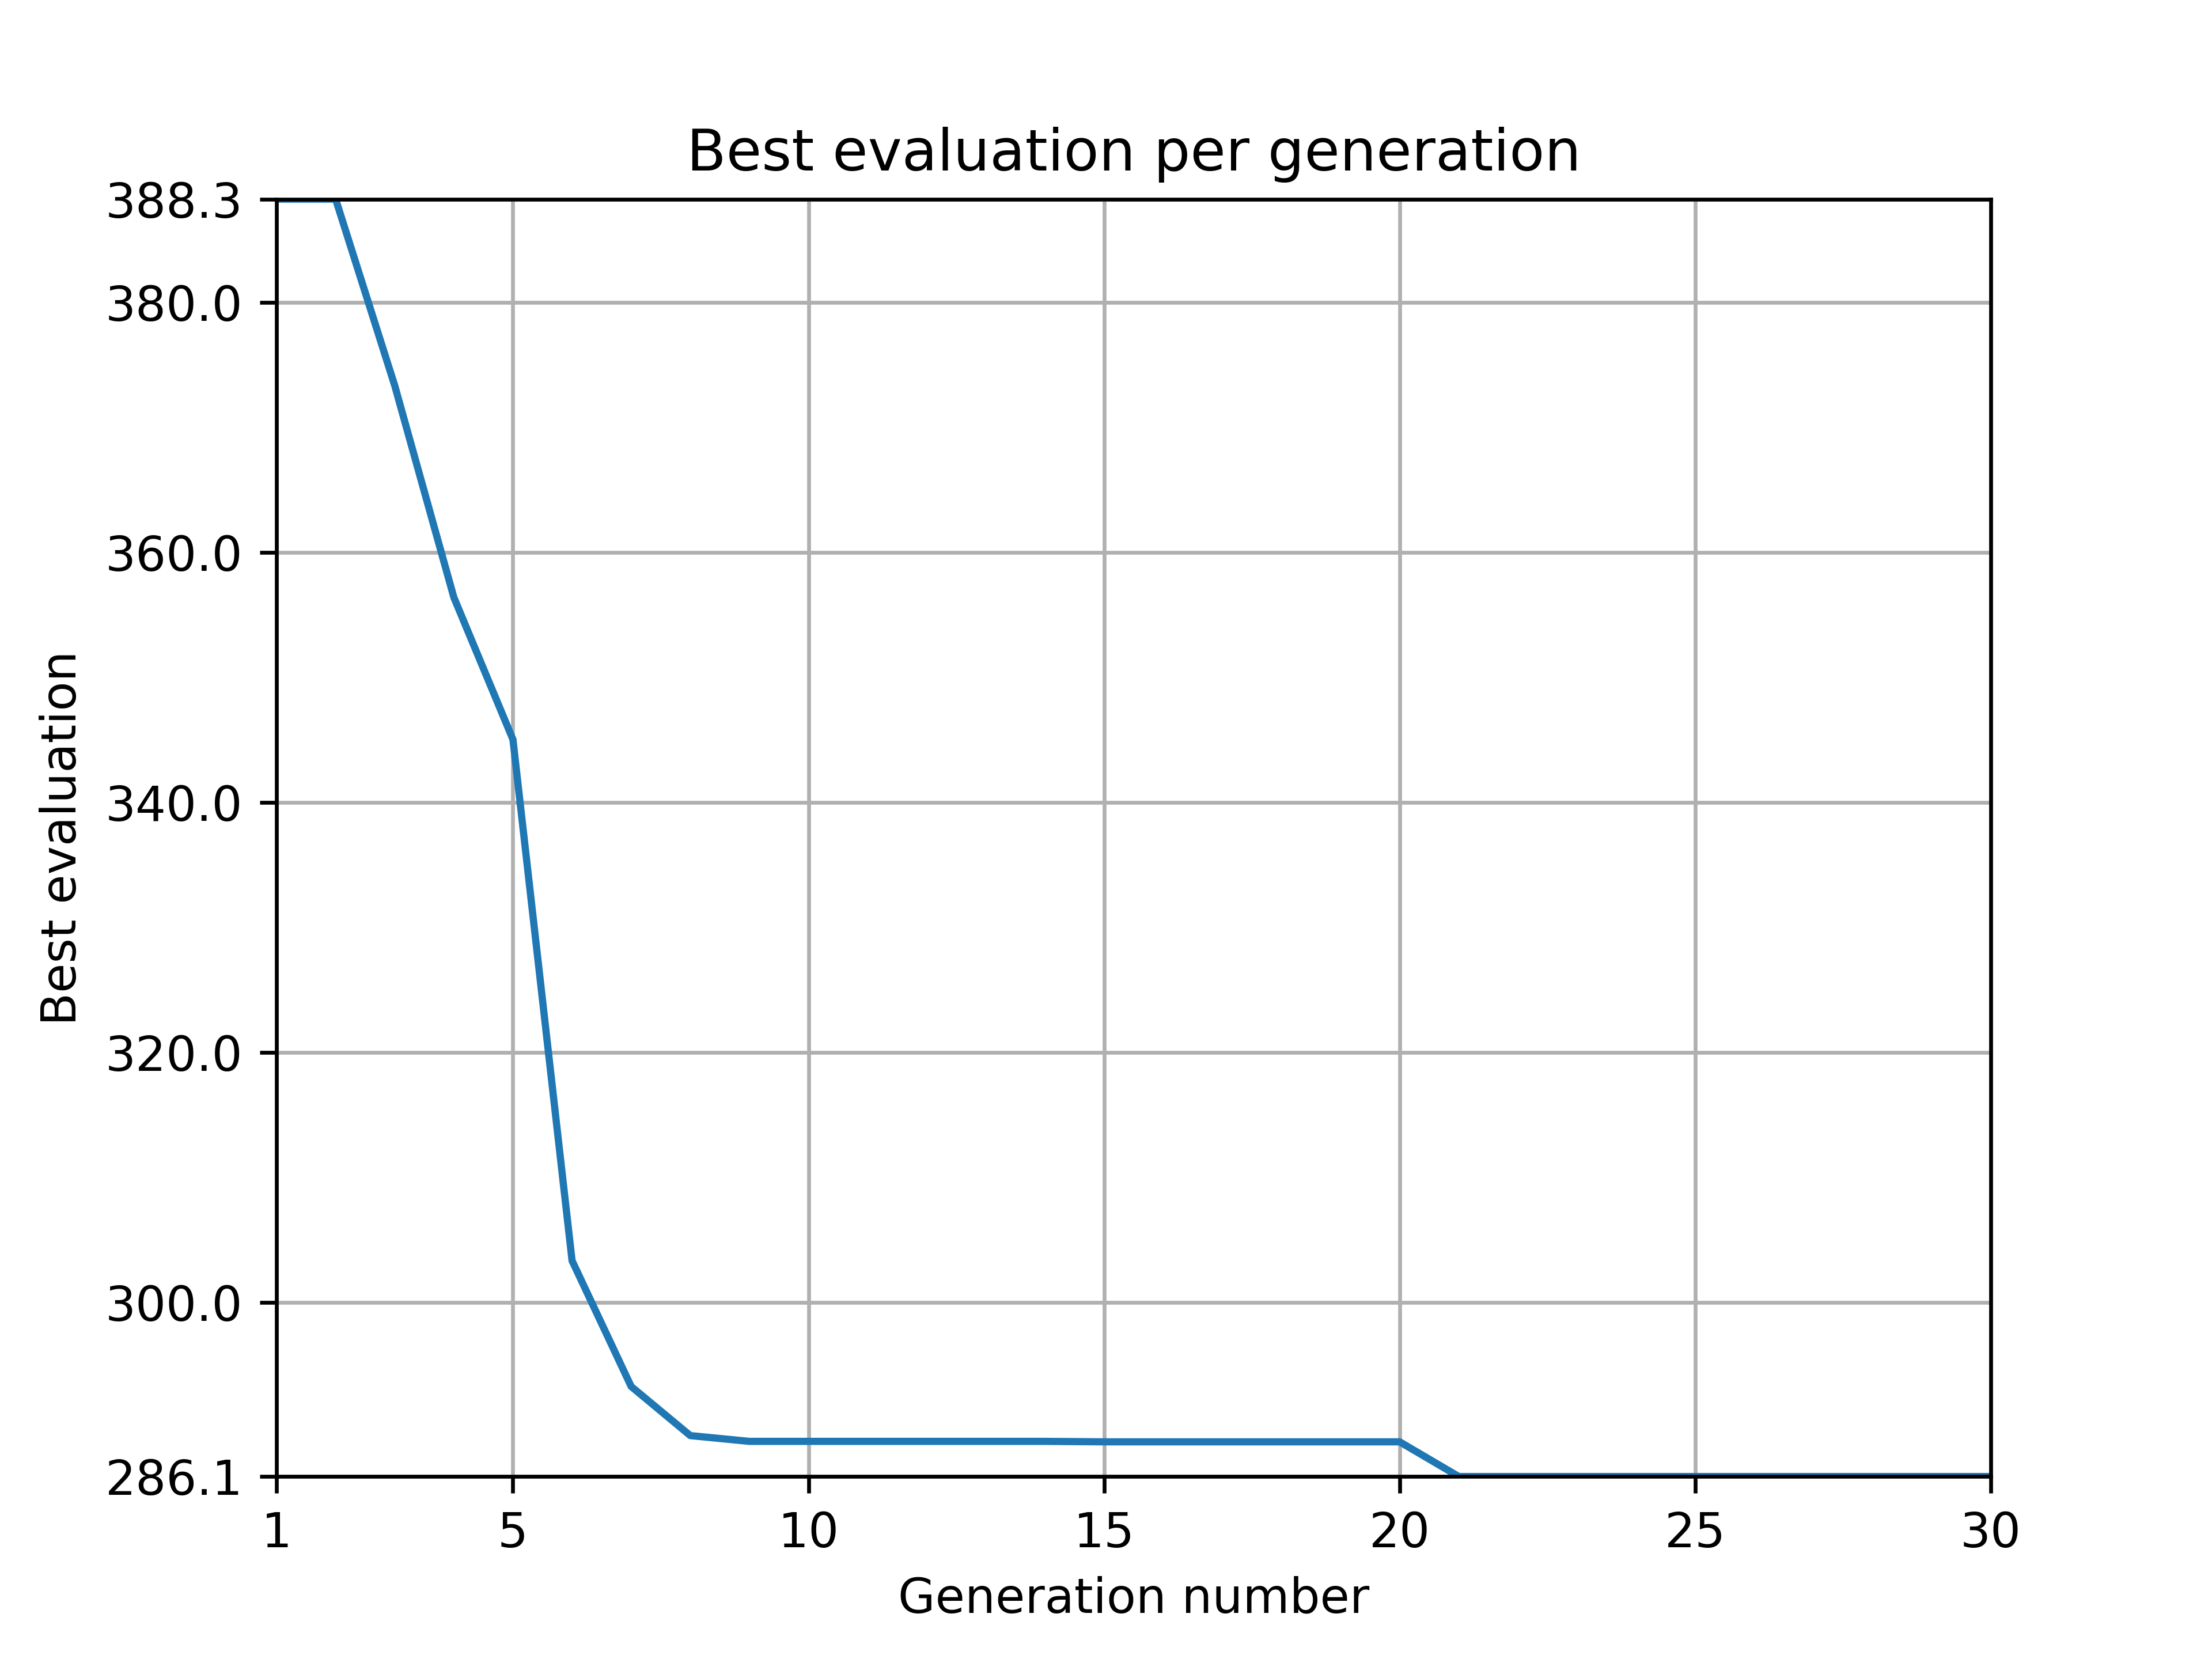
\includegraphics[width = \textwidth]{GeneticClustering_London_Evaluations}
    \caption{Line graph showing the best evaluation for each generation of clusters evolution process.}
    \label{fig:GeneticClustering_London_Evaluations}
\end{figure}
\noindent

\todo{Discuss why chosen, no clue what to put here, I just did it bc it's cool.}

\subsubsection{Centroid-based Genetic Clustering}
Inspired by K-Means, centroid-based genetic clustering uses a genetic algorithm to find the best set of centroids
to cluster the data.
The same process of evolution is used, as described previously, except this time the genome will specify the
centroids to use for clustering.
With a different genome structure, we will have to reconsider our crossover and mutation methods.
Centroid based genetic clustering keeps the same time complexity as genetic clustering, $O(g p r)$, with $g$ being the
number of generations, $p$ being the population size and $r$ being the time complexity of the chosen routing.\\
\todo{Figure out how to cite time complexity of genetic algorithms. Or go into explanation for our implementation.}

\noindent
Our new genome will be a list of coordinate pairs, representing the latitude and longitude of each centroid.
Figure~\ref{fig:GeneticCentroids_Greenwich_Example} shows an example of how locations are clustered using our centroid-based genome.
\begin{figure}[H]
    \centering
    Genome: $\begin{bmatrix}0.00 & 0.01 & -0.01 & 0.00 & 0.00\\51.477 & 51.477 & 51.477 & 51.482 & 51.472\end{bmatrix}$
    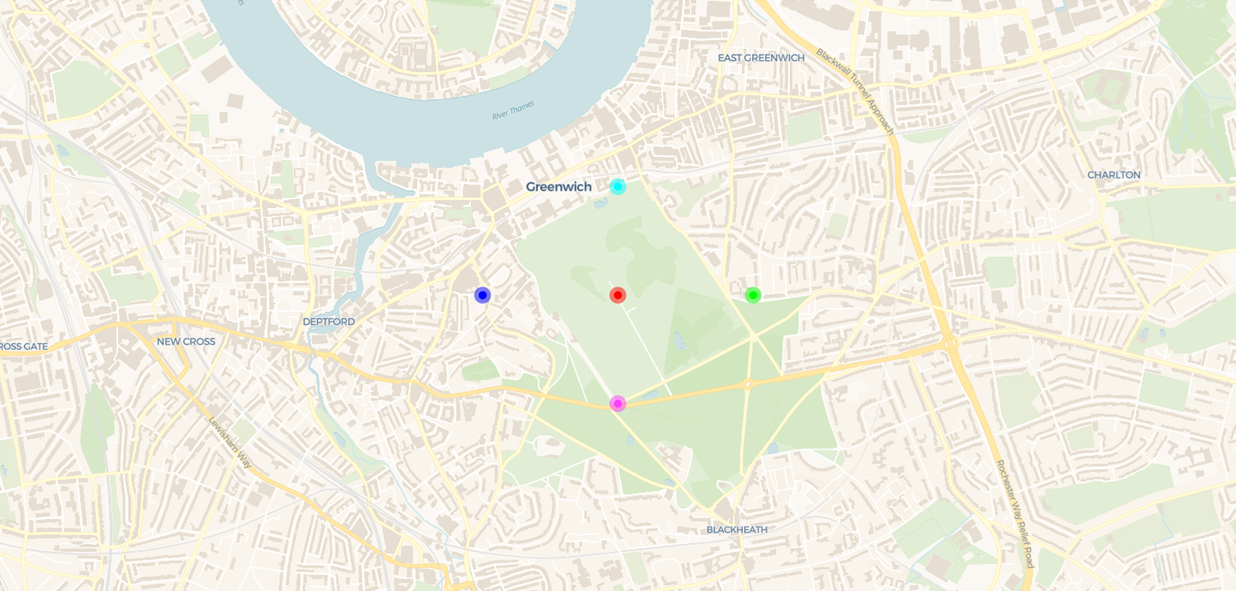
\includegraphics[width = \textwidth]{GeneticCentroids_Greenwich_Example}
    \caption{Example of how an individual's genome corresponds to cluster centroids.}
    \label{fig:GeneticCentroids_Greenwich_Example}
\end{figure}

\noindent
Once again, we will iteratively evolve our population through the process of selection, crossover and mutation.
Our selection procedure is largely the same in that we evaluate each individual by generating a trip with the help
of its genome and calculating the associated cost of these trips.
The only difference is that, because our genome is no longer a direct assignment of clusters, we first need to
assign each location to its nearest centroid.
This is shown in figure~\ref{fig:GeneticCentroids._evaluate_population}.
\begin{figure}[H]
    \centering
    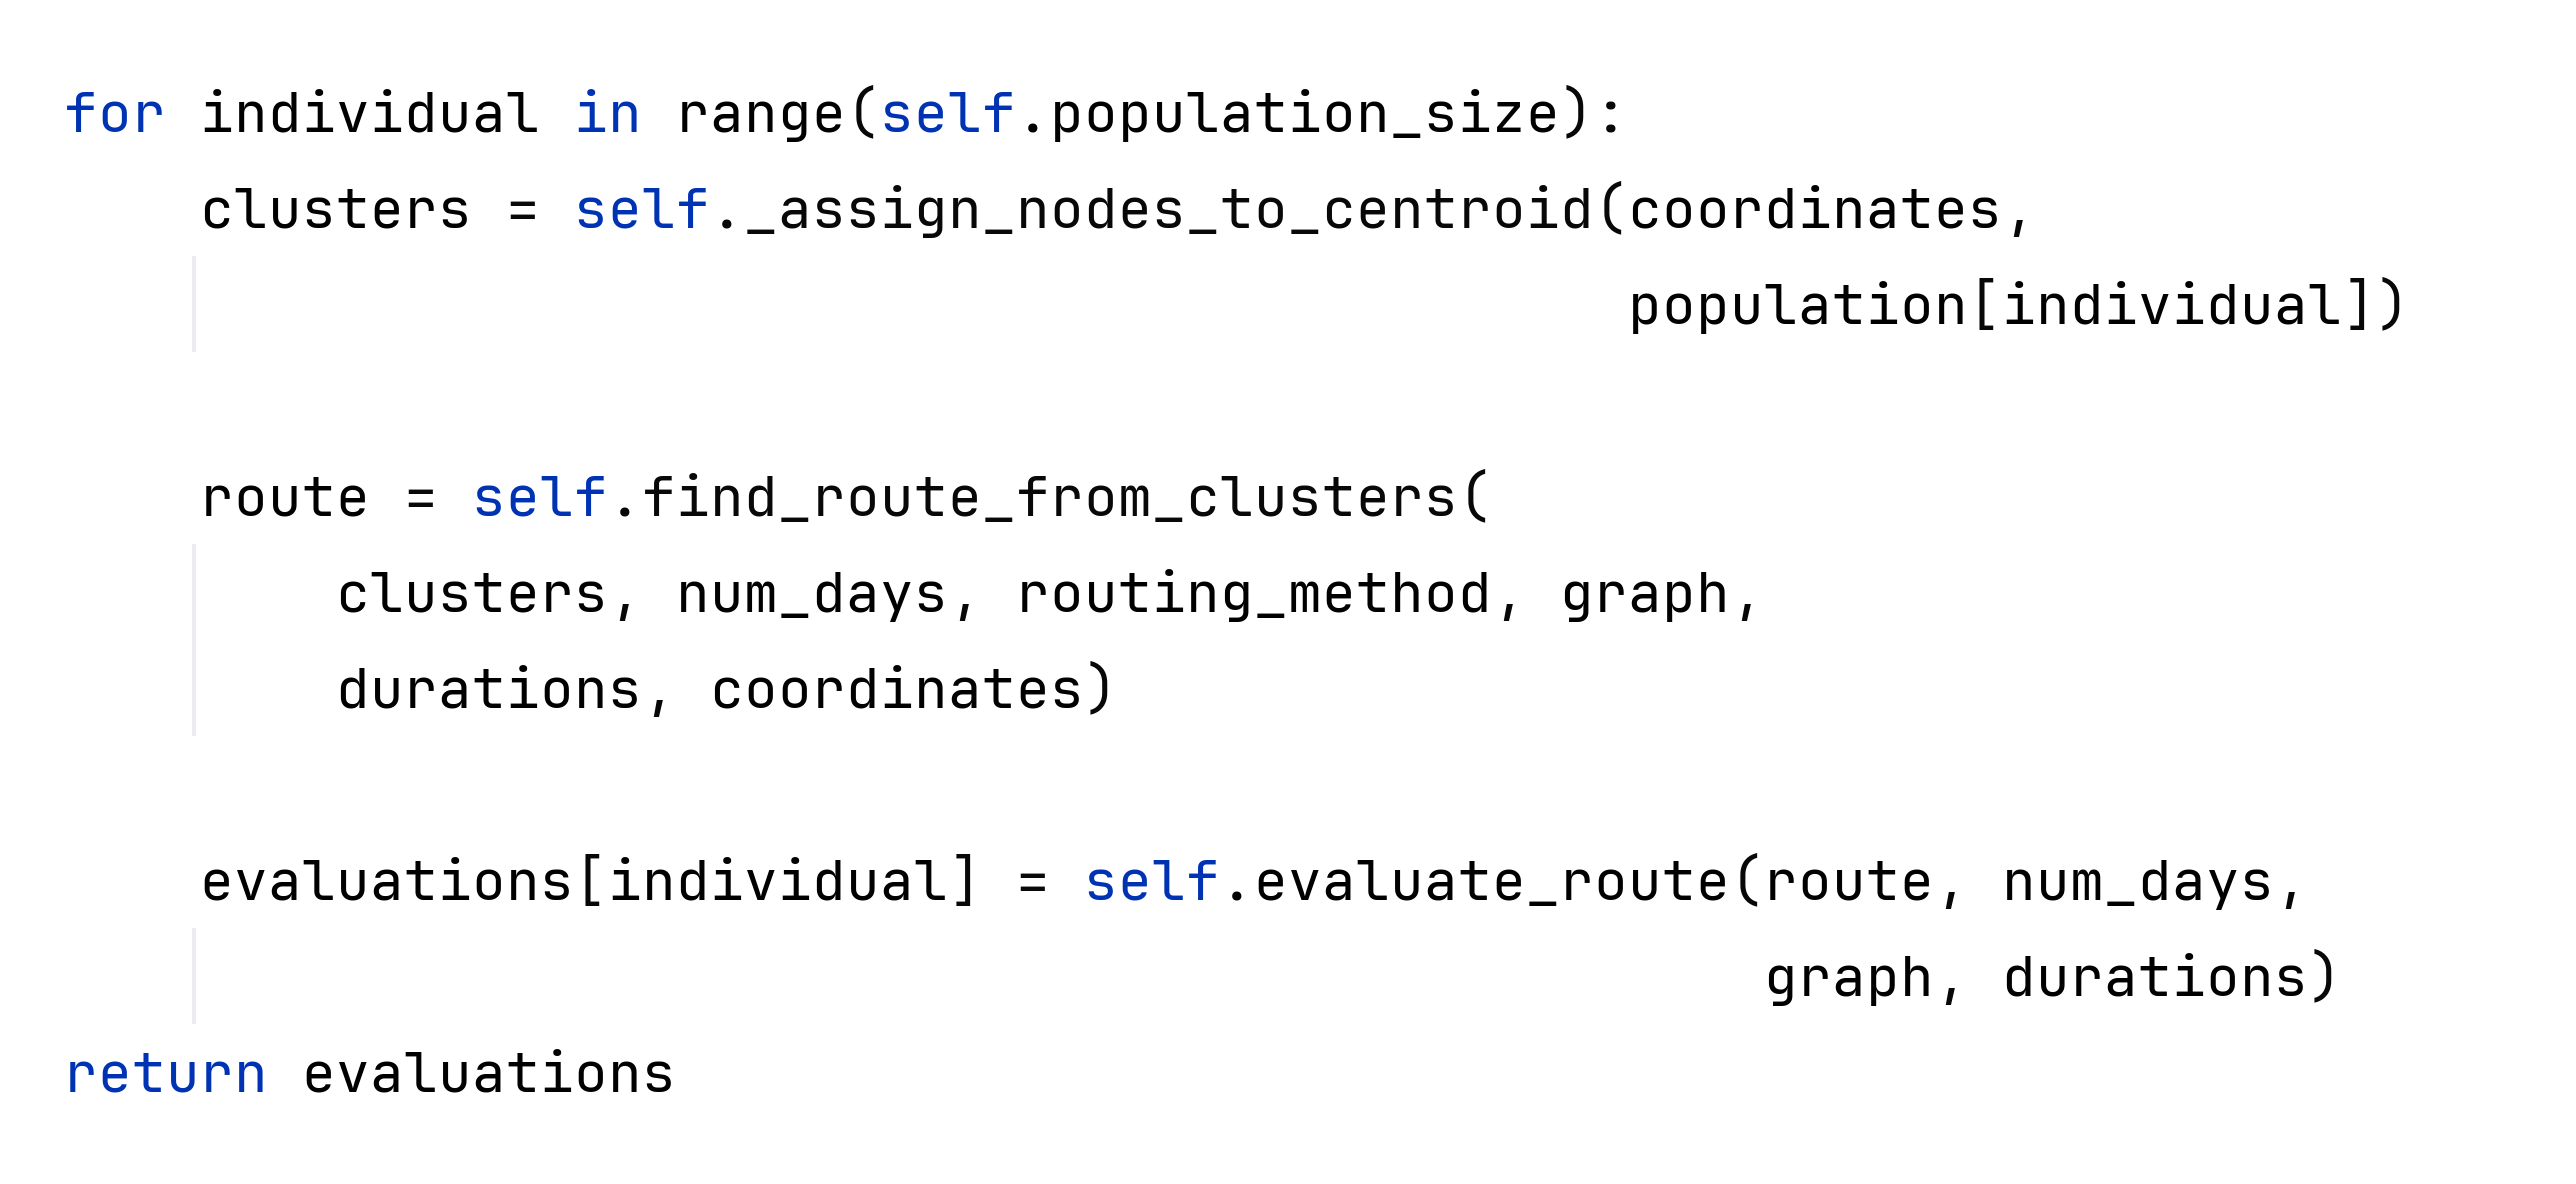
\includegraphics[width = \textwidth]{GeneticCentroids._evaluate_population}
    \caption{From GeneticCentroidClustering.\_evaluate\_population in algorithms\textbackslash clustering.py}
    \label{fig:GeneticCentroids._evaluate_population}
\end{figure}

\noindent
The `\_assign\_nodes\_to\_centroid' method shown in figure~\ref{fig:GeneticCentroids._evaluate_population} is the same
method we used for K-Means, shown in figure~\ref{fig:Clustering._assign_nodes_to_centroid}.
With the population evaluated we can select the best individuals for use in creating the next generation.
To create the next generation we enact the same stages of copying over the best individuals, generating some new
individual's randomly and creating the rest via crossover and mutation.

For this implementation of crossover, instead of selecting random genes from each parent, we will be taking the
values of both parents and merging them together.
In practice, this means taking the coordinates of each centroid from both parents and finding a point between them
to generate a new centroid.
How close this new centroid is to each parent is determined by generating a random weight, indicating how much
influence each parent has on the offspring.
\todo{Create and insert drawing of merging parent centroids}

\noindent
Similarly to the previous implementation of crossover, we need to reorder the centroids to ensure that both parents
are consistent with each other.
This time, because are genome isn't formed of discrete values we can rename, we will instead take an approach of
finding the most similar centroids from each parent and merging them.
This is performed by calculating the distances between each of parent 1s centroids to each of parent 2s, and
reordering the genome to place the closest centroids together.
Figure~\ref{fig:GeneticCentroids._crossover} shows this implementation of crossover, including how parents are
reordered and merged together to produce offspring.
\begin{figure}[H]
    \centering
    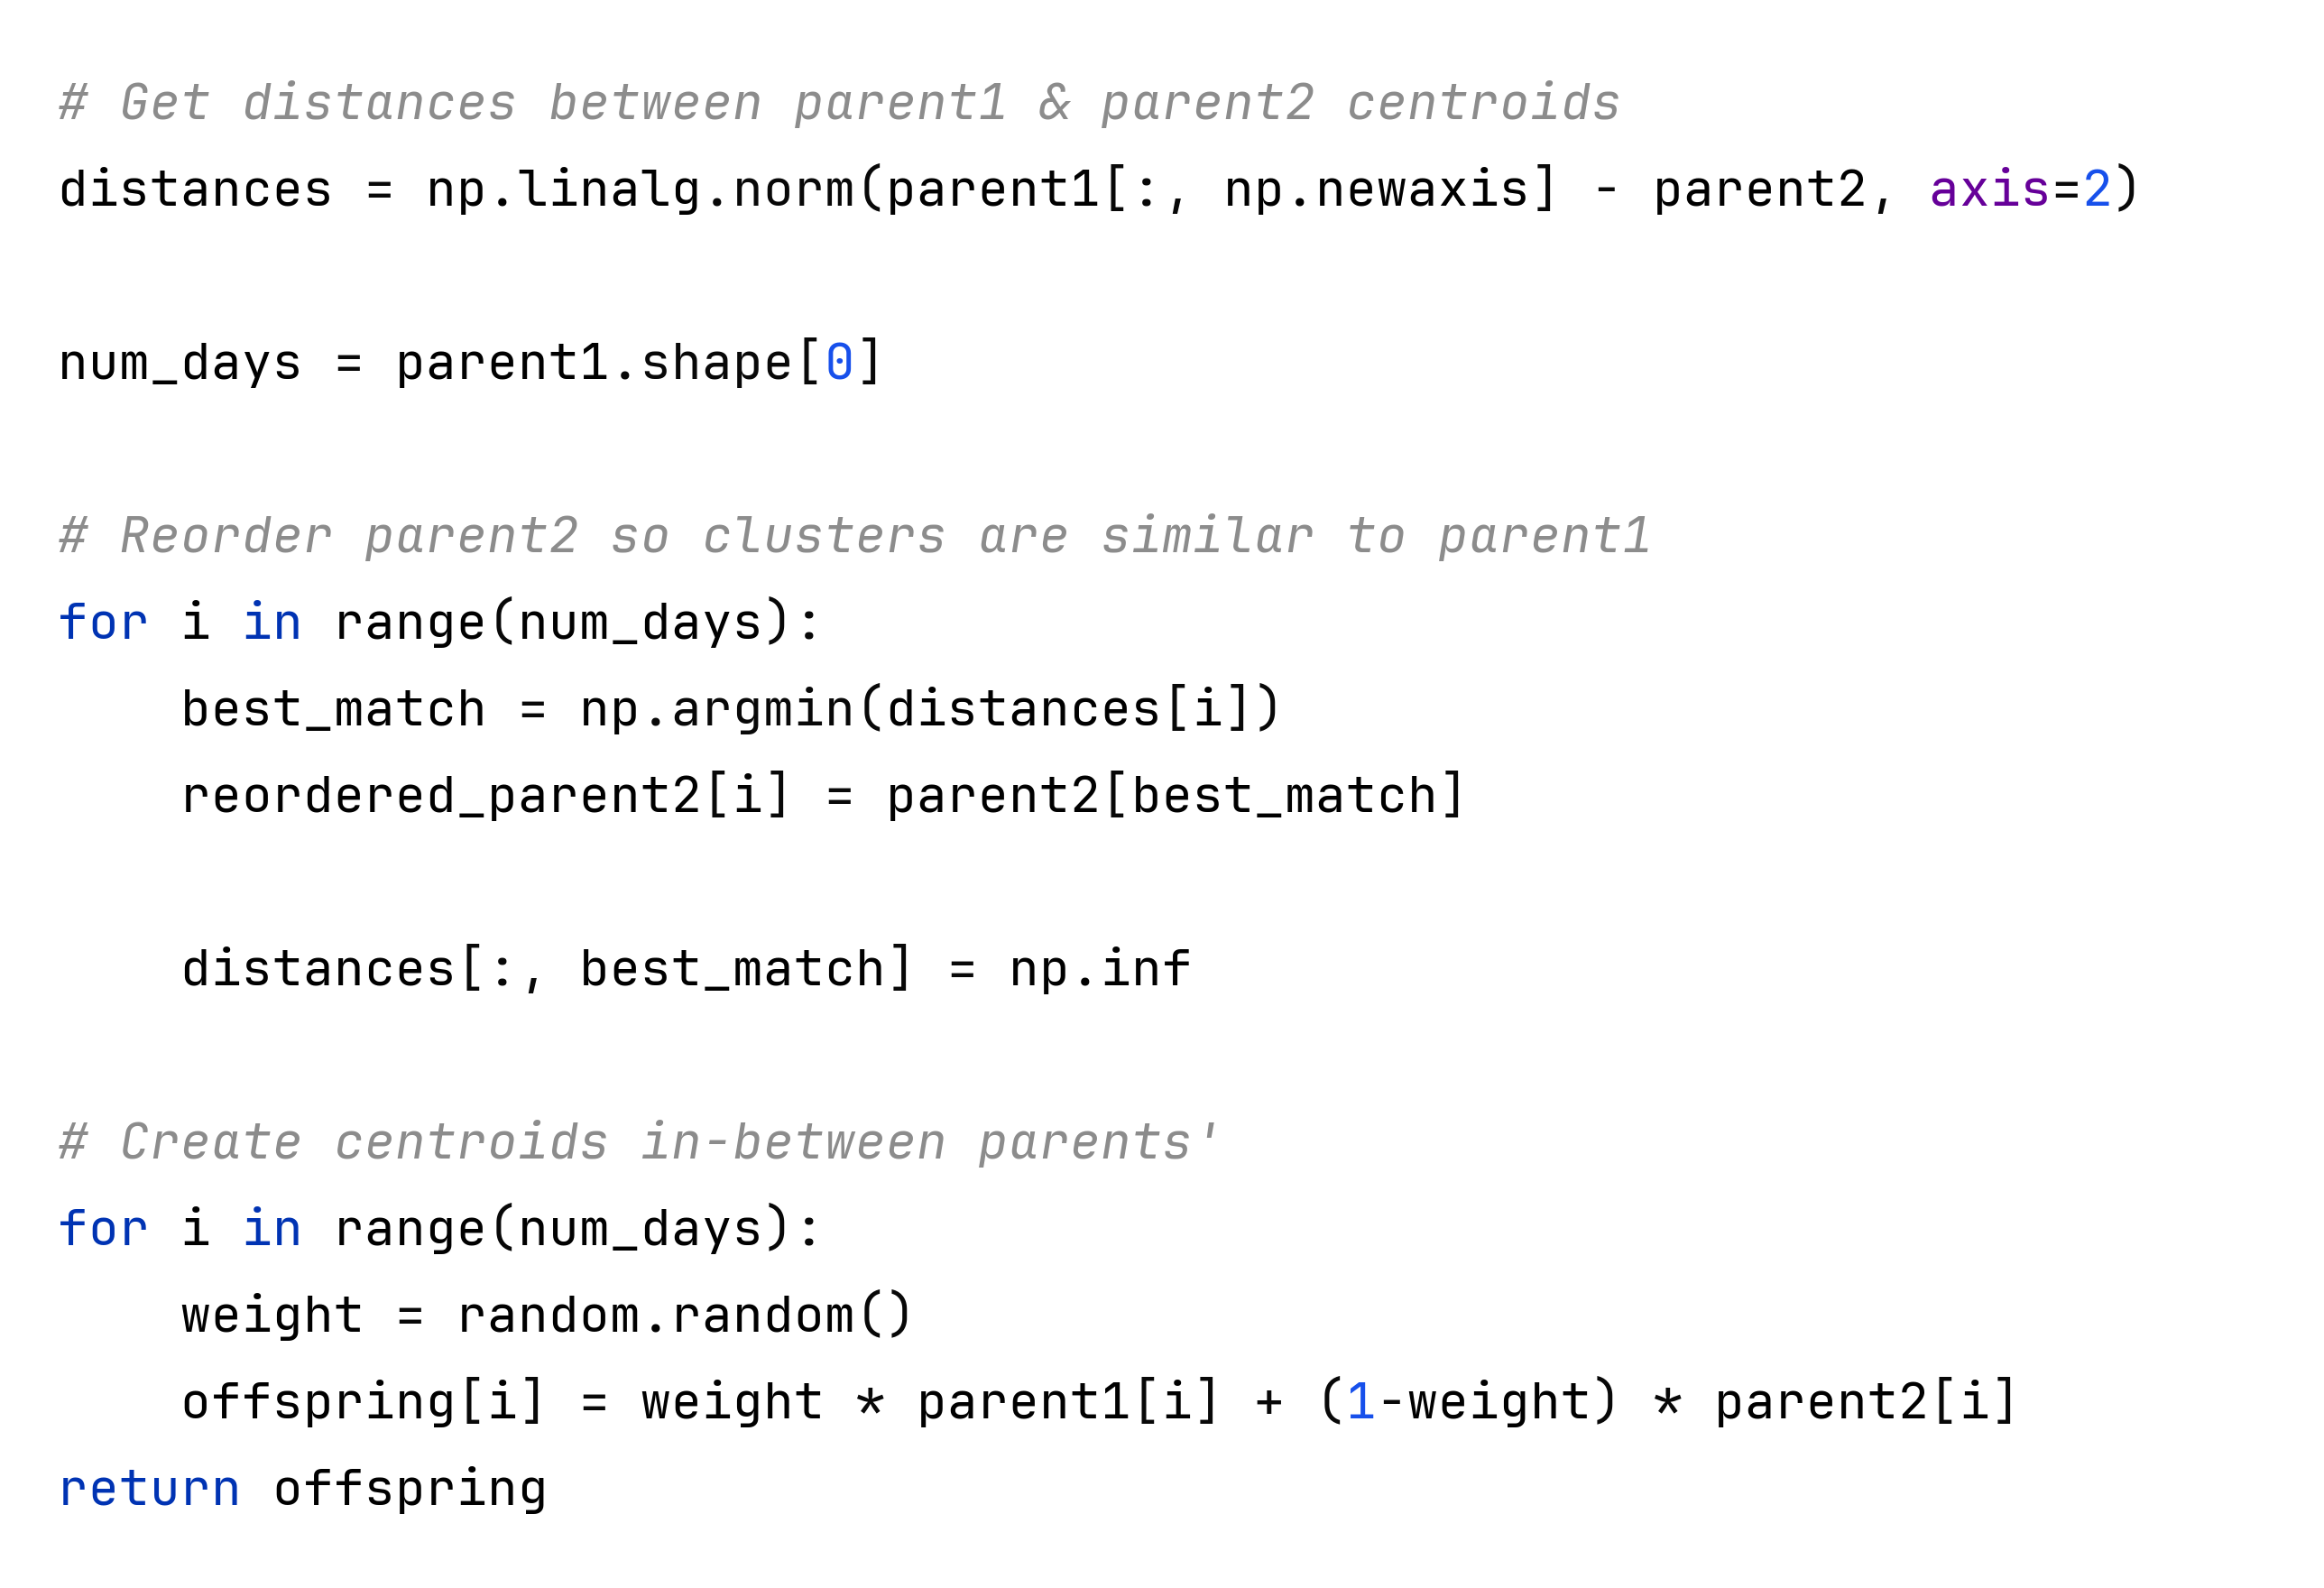
\includegraphics[width = \textwidth]{GeneticCentroids._crossover}
    \caption{Code from GeneticCentroidClustering.\_crossover in algorithms\textbackslash clustering.py}
    \label{fig:GeneticCentroids._crossover}
\end{figure}

\noindent
For mutation, we will go through each centroid of each individual and randomly decide if it will mutate or not.
If a centroid is chosen to mutate, we will randomly select a new location for it within the bound of the input
coordinates.
The minimum and maximum latitude and longitude of the input are used to form a region within which new centroids can
be generated, ensuring that the mutation is still relevant to the input.
Figure~\ref{fig:GeneticCentroids.find_clusters.mutation} shows this process of mutation.
\begin{figure}[H]
    \centering
    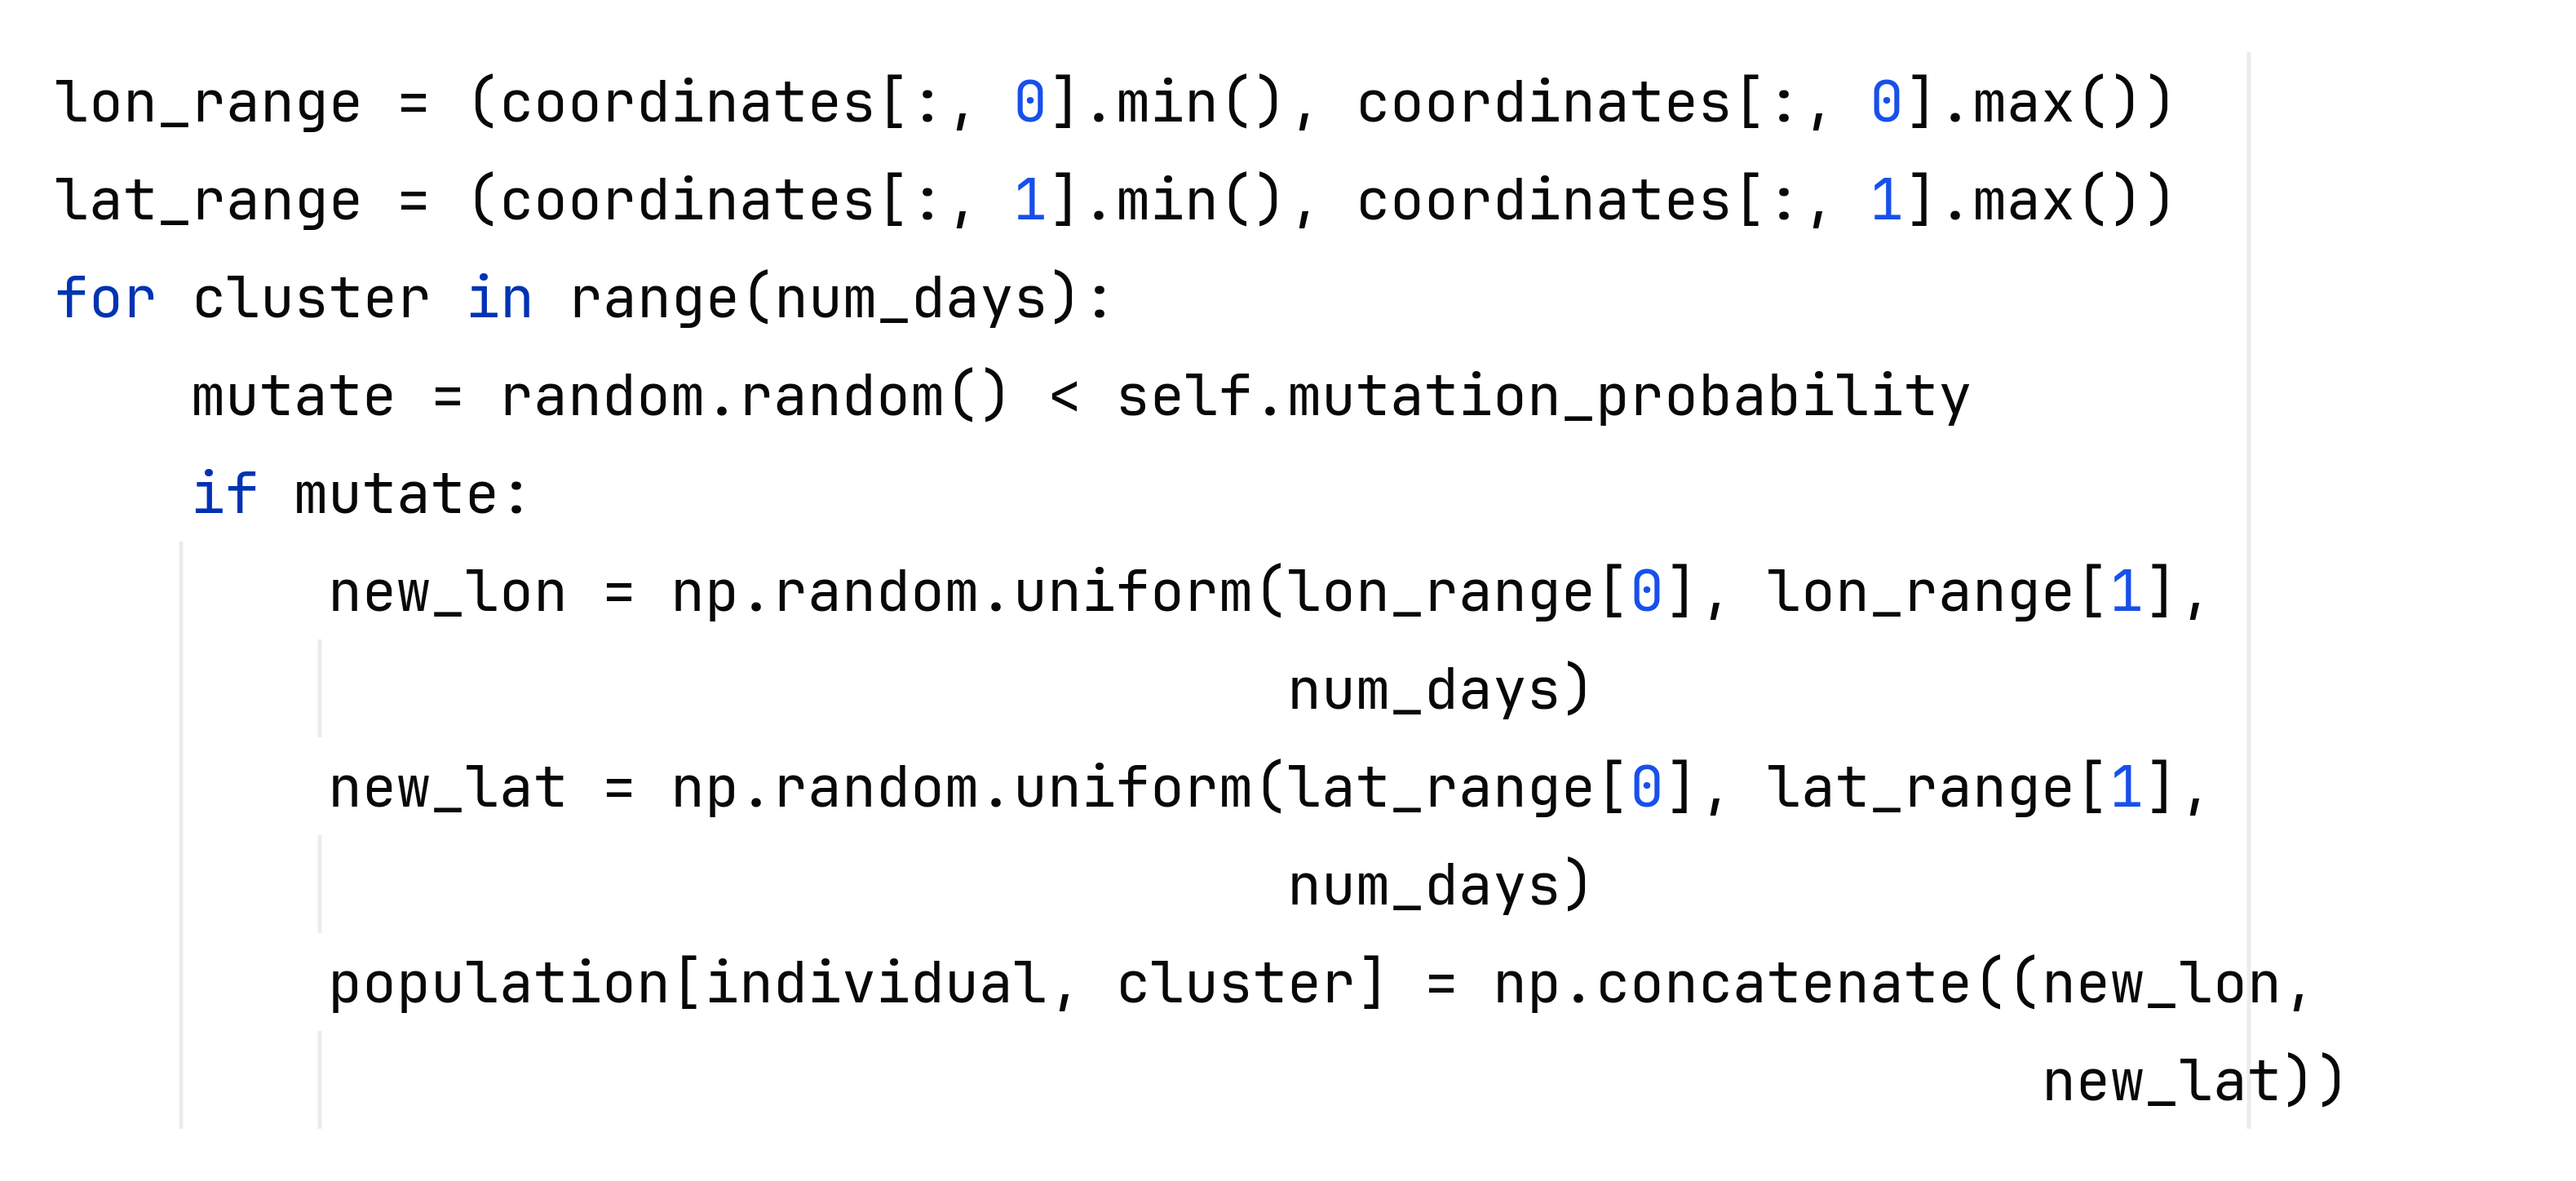
\includegraphics[width = \textwidth]{GeneticCentroids.find_clusters.mutation}
    \caption{Code from GeneticCentroidClustering.find\_clusters in algorithms\textbackslash clustering.py}
    \label{fig:GeneticCentroids.find_clusters.mutation}
\end{figure}

\noindent
Once again, this process of selection, crossover and mutation is repeated until a maximum number of generations is reached.
By the end of this process, we will have a population of individuals that have been evolved to find good centroids
for clustering the input.
Figure~\ref{fig:GeneticCentroids_London_Generation1} shows an example of genetic centroid-based clustering using the same
input as for previous clustering examples.
This example of genetic centroid-based clustering used the same hyperparameters as the previous genetic clustering
example, evolving 30 generations with a population size of 12, a crossover rate of 0.9, a mutation rate of 0.1 and
once again using greedy routing alongside our clustering to produce trips.
Again, a line graph of the best evaluation found for each generation of the process, this is shown in
figure~\ref{fig:GeneticCentroids_London_Evaluations}.
\begin{figure}[H]
    \ContinuedFloat*
    \centering
    \includegraphics[width = \textwidth]{GeneticCentroids_London_Generation1}
    \caption{Genetic Centroid Clustering example, best route found in Generation 1.}
    \label{fig:GeneticCentroids_London_Generation1}
\end{figure}
\begin{figure}[H]
    \ContinuedFloat
    \centering
    \includegraphics[width = \textwidth]{GeneticCentroids_London_Generation5}
    \caption{Genetic Centroids Clustering example, best route found in Generation 5.}
    \label{fig:GeneticCentroids_London_Generation5}
\end{figure}
\begin{figure}[H]
    \ContinuedFloat
    \centering
    \includegraphics[width = \textwidth]{GeneticCentroids_London_Generation10}
    \caption{Genetic Centroids Clustering example, best route found in Generation 10.}
    \label{fig:GeneticCentroids_London_Generation10}
\end{figure}
\begin{figure}[H]
    \ContinuedFloat
    \centering
    \includegraphics[width = \textwidth]{GeneticCentroids_London_Generation30}
    \caption{Genetic Centroids Clustering example, best route found in Generation 30, evolution is now complete.}
    \label{fig:GeneticCentroids_London_Generation30}
\end{figure}
\begin{figure}[H]
    \centering
    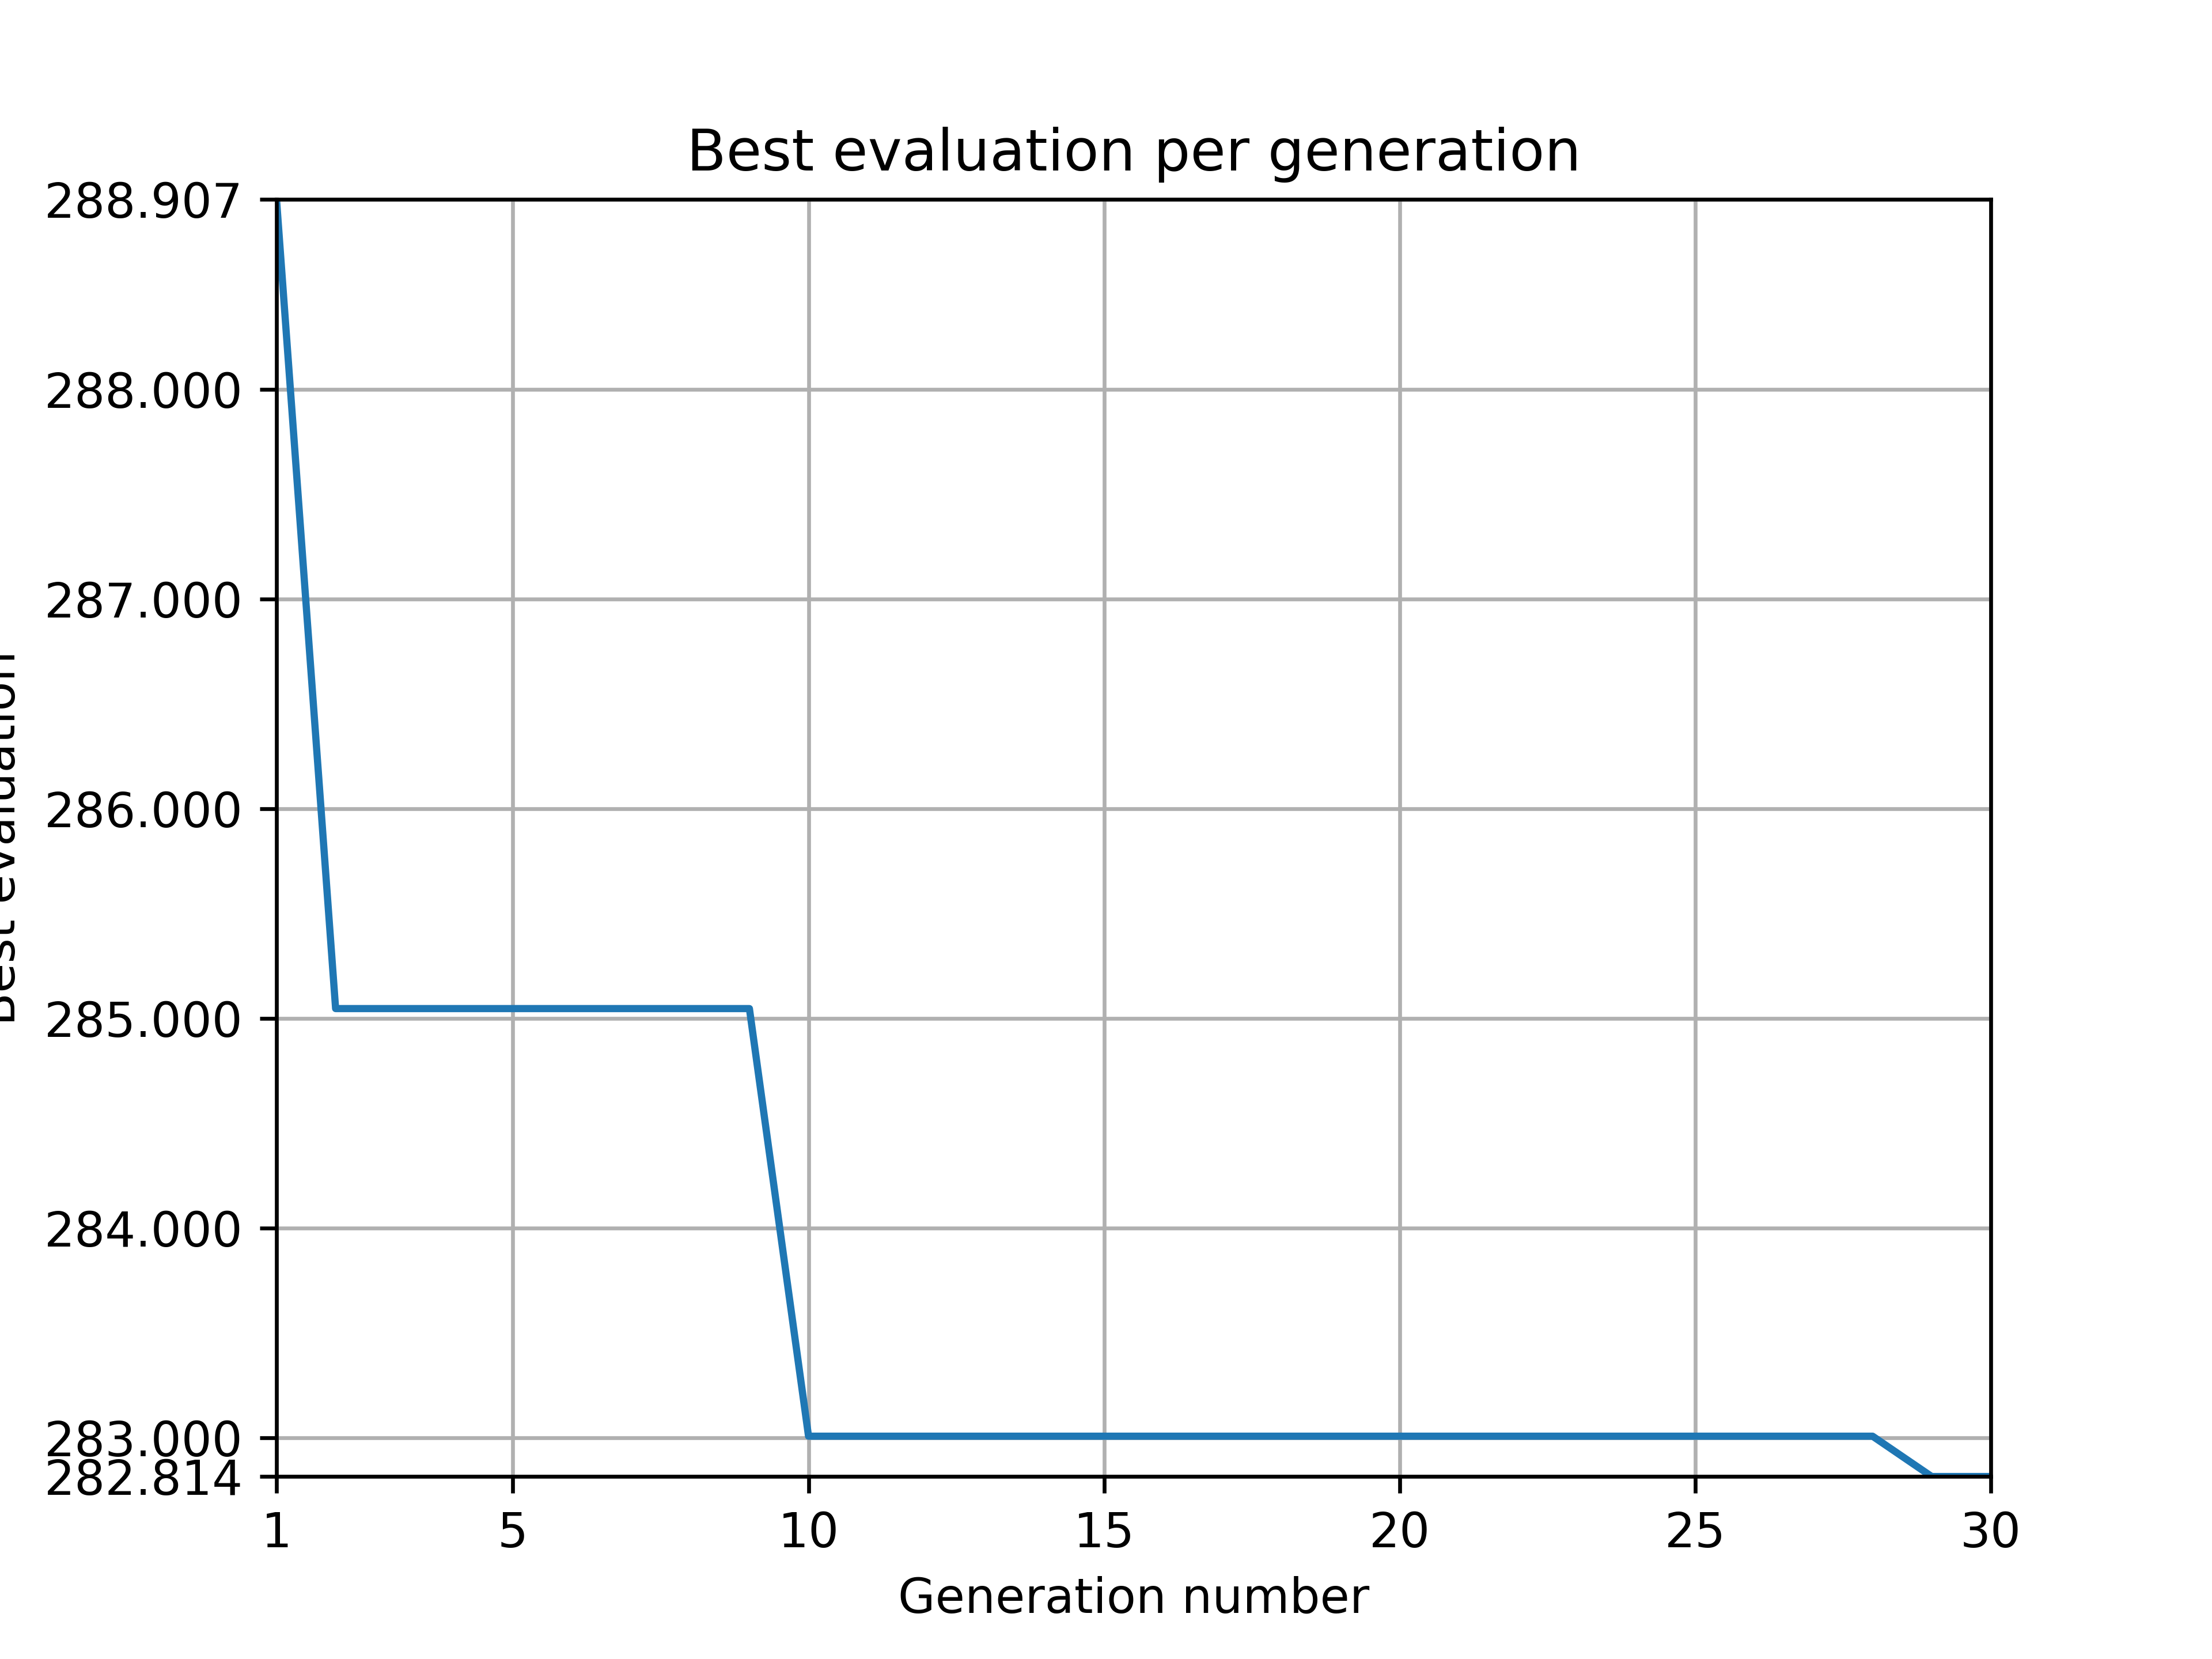
\includegraphics[width = \textwidth]{GeneticCentroids_London_Evaluations}
    \caption{Line graph showing the best evaluation for each generation of centroids evolution process.}
    \label{fig:GeneticCentroids_London_Evaluations}
\end{figure}
\noindent

\noindent
\todo{Discuss why chosen, to investigate how a k-means like approach would work with a genetic algorithm and whether regular clustering is better.}

\subsection{Routing}\label{subsec:routing}
The routing algorithms implemented in this project are TSP solvers, aiming to find a route with minimal travel time
that visits all given locations.
There are two ways in which routing will be used to form a trip either by using a clustering algorithm and then
finding a route for each cluster (as previously described in section~\ref{subsec:clustering}), or by finding a route
that visits every location, before splitting the route into multiple days (as will be described in section~\ref{subsec:route-insertion}).
The routing algorithms implemented in this project are: Brute Force, Greedy, Gift Wrapping and Genetic.

\subsubsection{Brute Force}\label{subsubsec:brute-force-routing}
Brute Force is an exhaustive algorithm that tries every possible route to find one with the least cost.
We find every route by generating all permutations of the locations to be visited, with the order of the locations
in each permutation representing the order in which they will be visited.
Each permutation is evaluated based on the amount of time it takes to travel the route, with the shortest route being
returned.
By checking every route Brute Force is guaranteed to find the best possible route, but has a time complexity of $O(n!)$.
\todo{Maybe cite time complexity of brute force or permutations of a set?}\\

\noindent
It's worth noting that in our implementation, since all routes must return to the starting point, the final location
of a route is fixed.
Therefore, we only need to consider $n-1$ locations, resulting in $(n-1)!$ possible permutations.
To check every route, we'll be creating a mapping between every integer $\{0, 1, \mathellipsis, (n-1!)-1\}$ to every
permutation.
For a given integer $k$, and a list of possible locations $L: \{0, 1, \mathellipsis, n-1\}$ we can calculate $k$'s
corresponding permutation through the following steps:
\begin{enumerate}
    \item Divide $k$ by $(n-2)$ to find $x_1: \{0\leq x<n-1\}$, and the remainder $r_1$.
    \item $x_1$ is used to select a location for $L$, which will be the first location in our permutation. $L_{x_1}$ is
    removed from L.
    \item Divide $r_1$ by $(n-3)!$ to find $x_2: \{0\leq x<n-2\}$, and the remainder $r_2$.
    \item $x_2$ is used to select another location from $L$, which will be the second location in our permutation.
    Again, $L_{x_2}$ is removed from L.
    \item Repeat this process until all locations are assigned a position.
\end{enumerate}

\noindent
To help explain this, an example is shown in figure~\ref{fig:permutation-calculation-example}, generating a
permutation $P$ of the set $L = \{a, b, c, d\}$ that maps to $k = 17$.
\begin{figure}[H]
    \textbf{Step 1:} Divide $k = 17$ by $(n-1)! = 3! = 6$\\
    $17 \div 6 = 2$ with remainder $5$. Thus $x_1 = 2, r_1 = 5$\\
    We select $L_{x_1} = L_2 = c$ as the first element of our permutation.\\
    Updated sets: $L = \{a, b, d\}, P = \{c\}$\\

    \textbf{Step 2:} Divide $r_1 = 5$ by $(n-2)! = 2! = 2$\\
    $5 \div 2 = 2$ with remainder $1$. Thus $x_2 = 2, r_2 = 1$\\
    We select $L_{x_2} = L_2 = d$ as the second element of our permutation.\\
    Updated sets: $L = \{a, b\}, P = \{c, d\}$\\

    \textbf{Step 3:} Divide $r_2 = 1$ by $(n-3)! = 1! = 1$\\
    $1 \div 1 = 1$ with remainder $0$. Thus, $x_3 = 1, r_3 = 0$\\
    We select $L_{x_3} = L_1 = b$ as the third element of our permutation.\\
    Updated sets: $L = \{a\}, P = \{c, d, b\}$\\

    \textbf{Step 4:} There's only one element left, so $a$ becomes the last element.\\
    Updated sets: $P = \{c, d, b, a\}$
    \caption{Example of generating a permutation of a set using an integer mapping}
    \label{fig:permutation-calculation-example}
\end{figure}

\noindent
This method ensures that each integer maps to a unique permutation, allowing us to check every possible route.
Our python version of this is shown in figure~\ref{fig:Algorithm.generate_route}.
\begin{figure}[H]
    \centering
    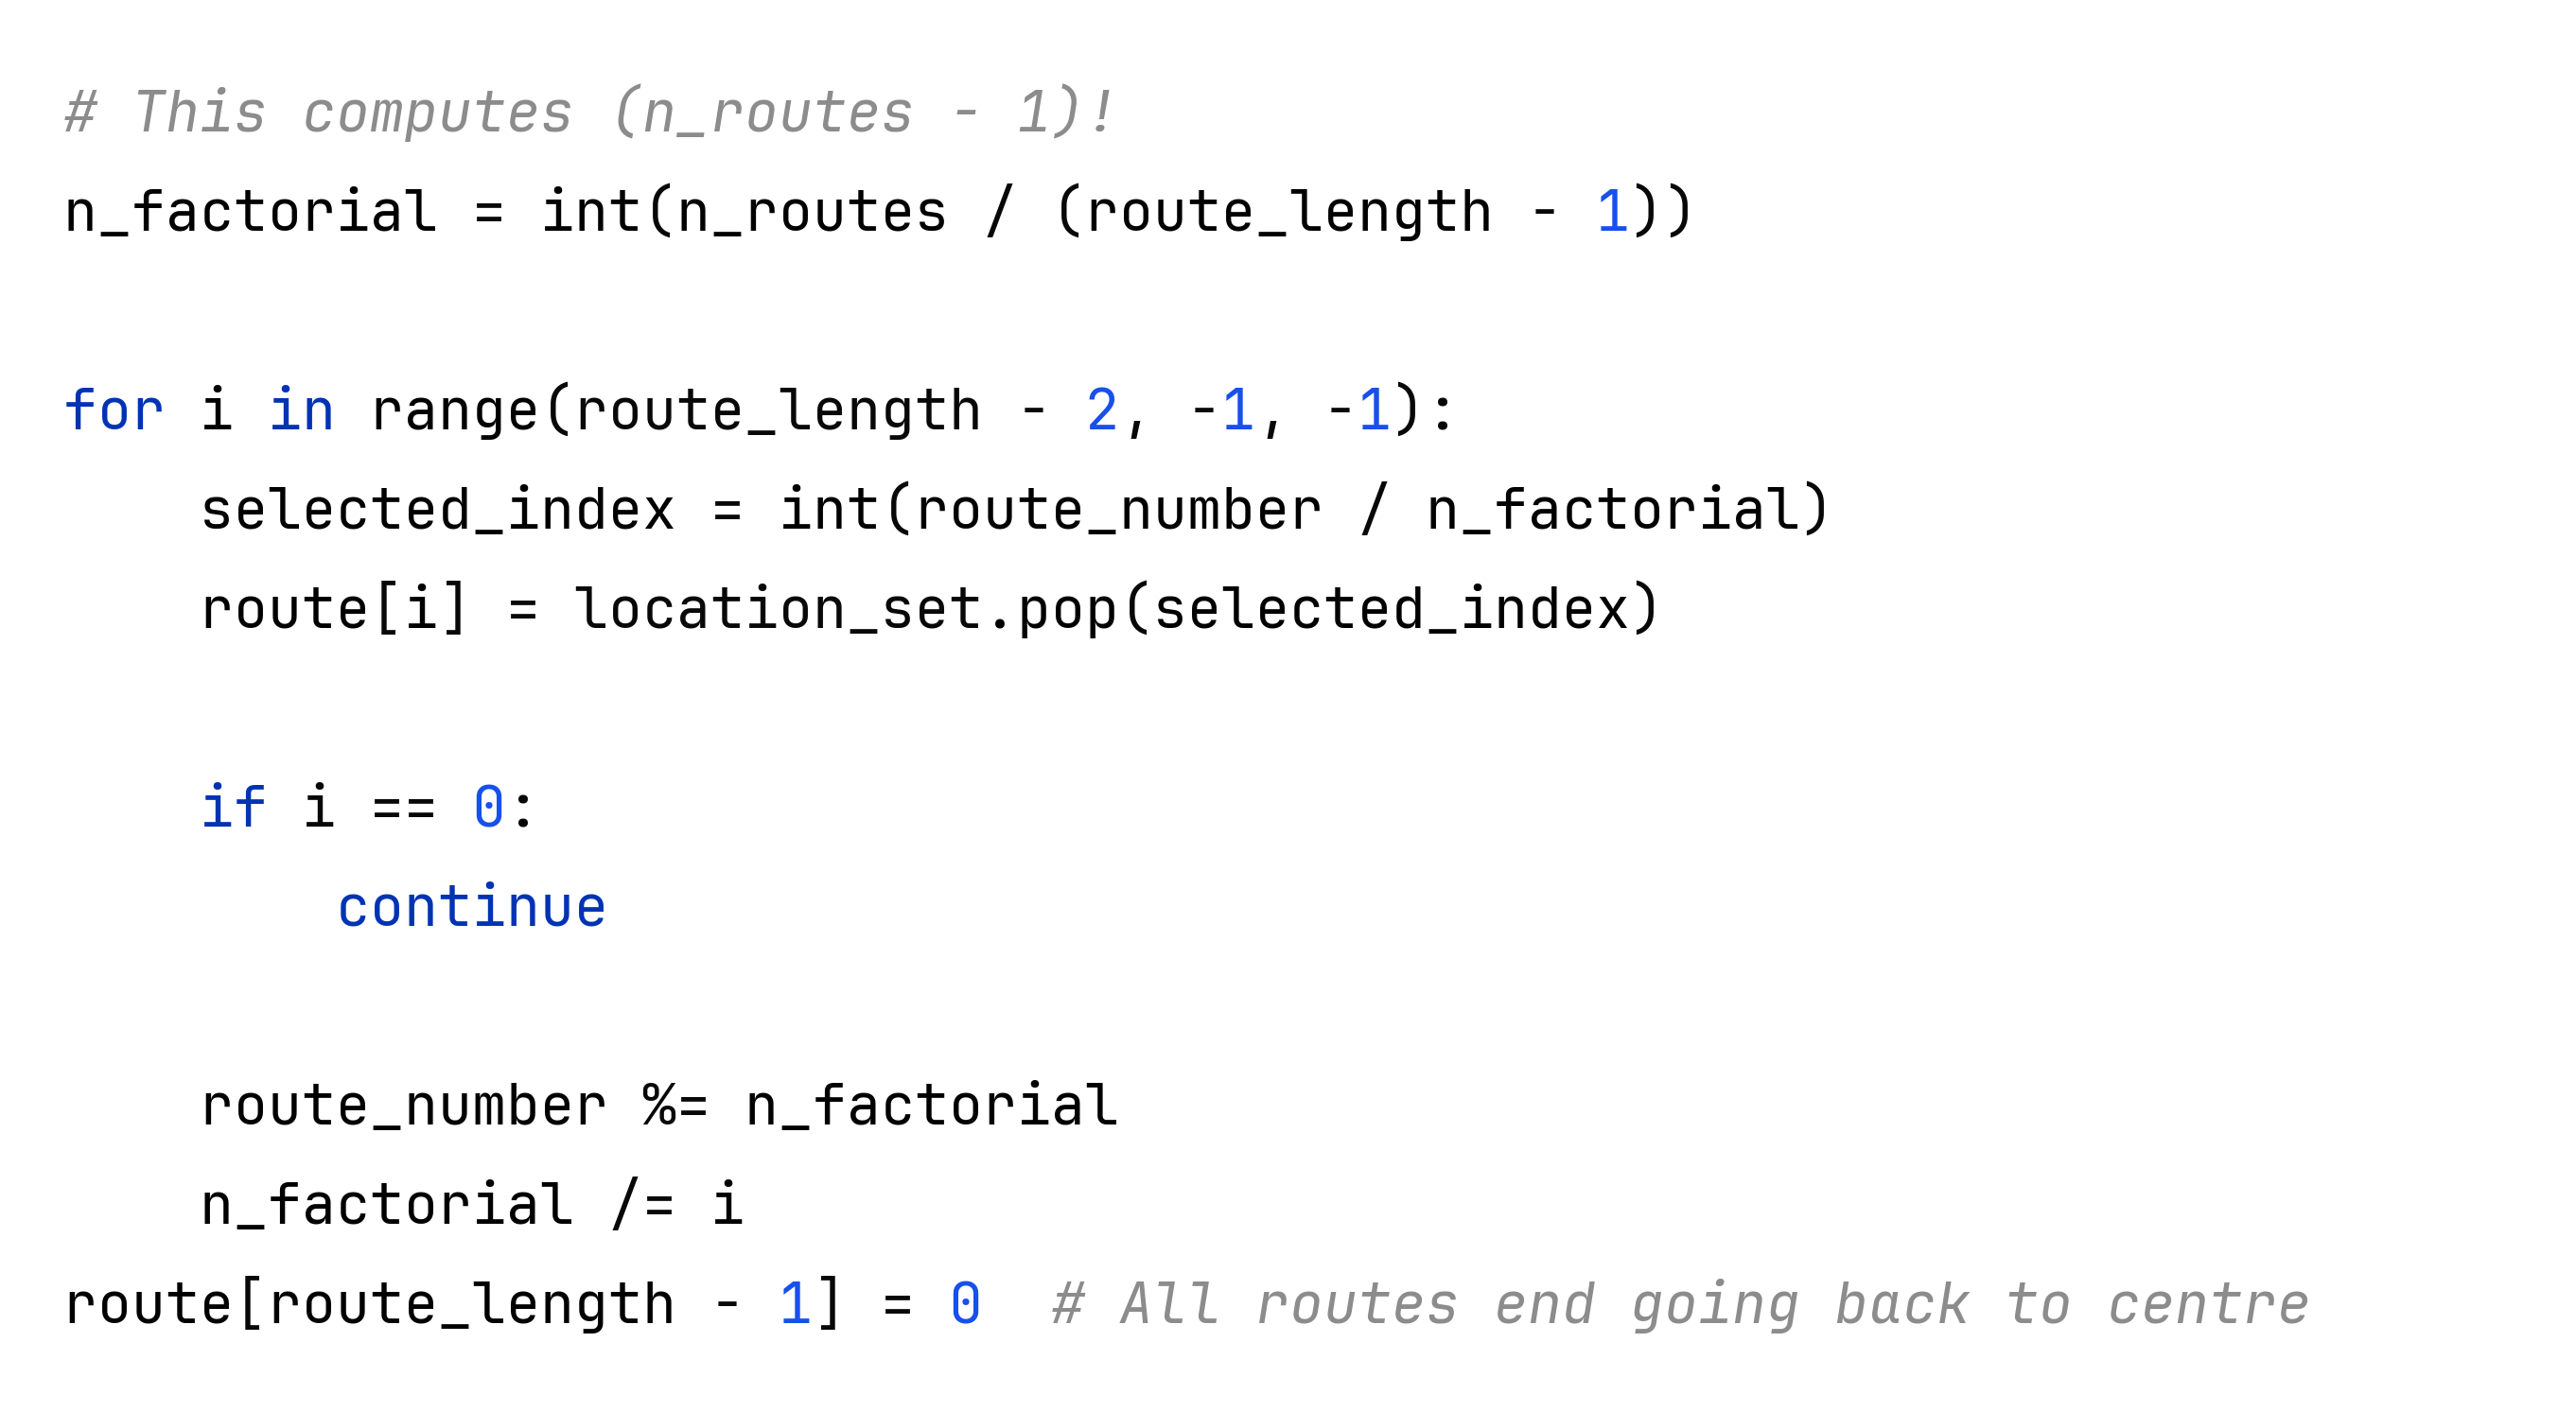
\includegraphics[width = \textwidth]{Algorithm.generate_route}
    \caption{Code from Algorithm.generate\_route in algorithms\textbackslash algorithm.py}
    \label{fig:Algorithm.generate_route}
\end{figure}

\noindent
With this method of generating routes in place, we just need to iterate through them all, evaluate them, and keep
track of the best found.
Our implementation of this is shown in figure~\ref{fig:Routing.brute_force}.
\begin{figure}[H]
    \centering
    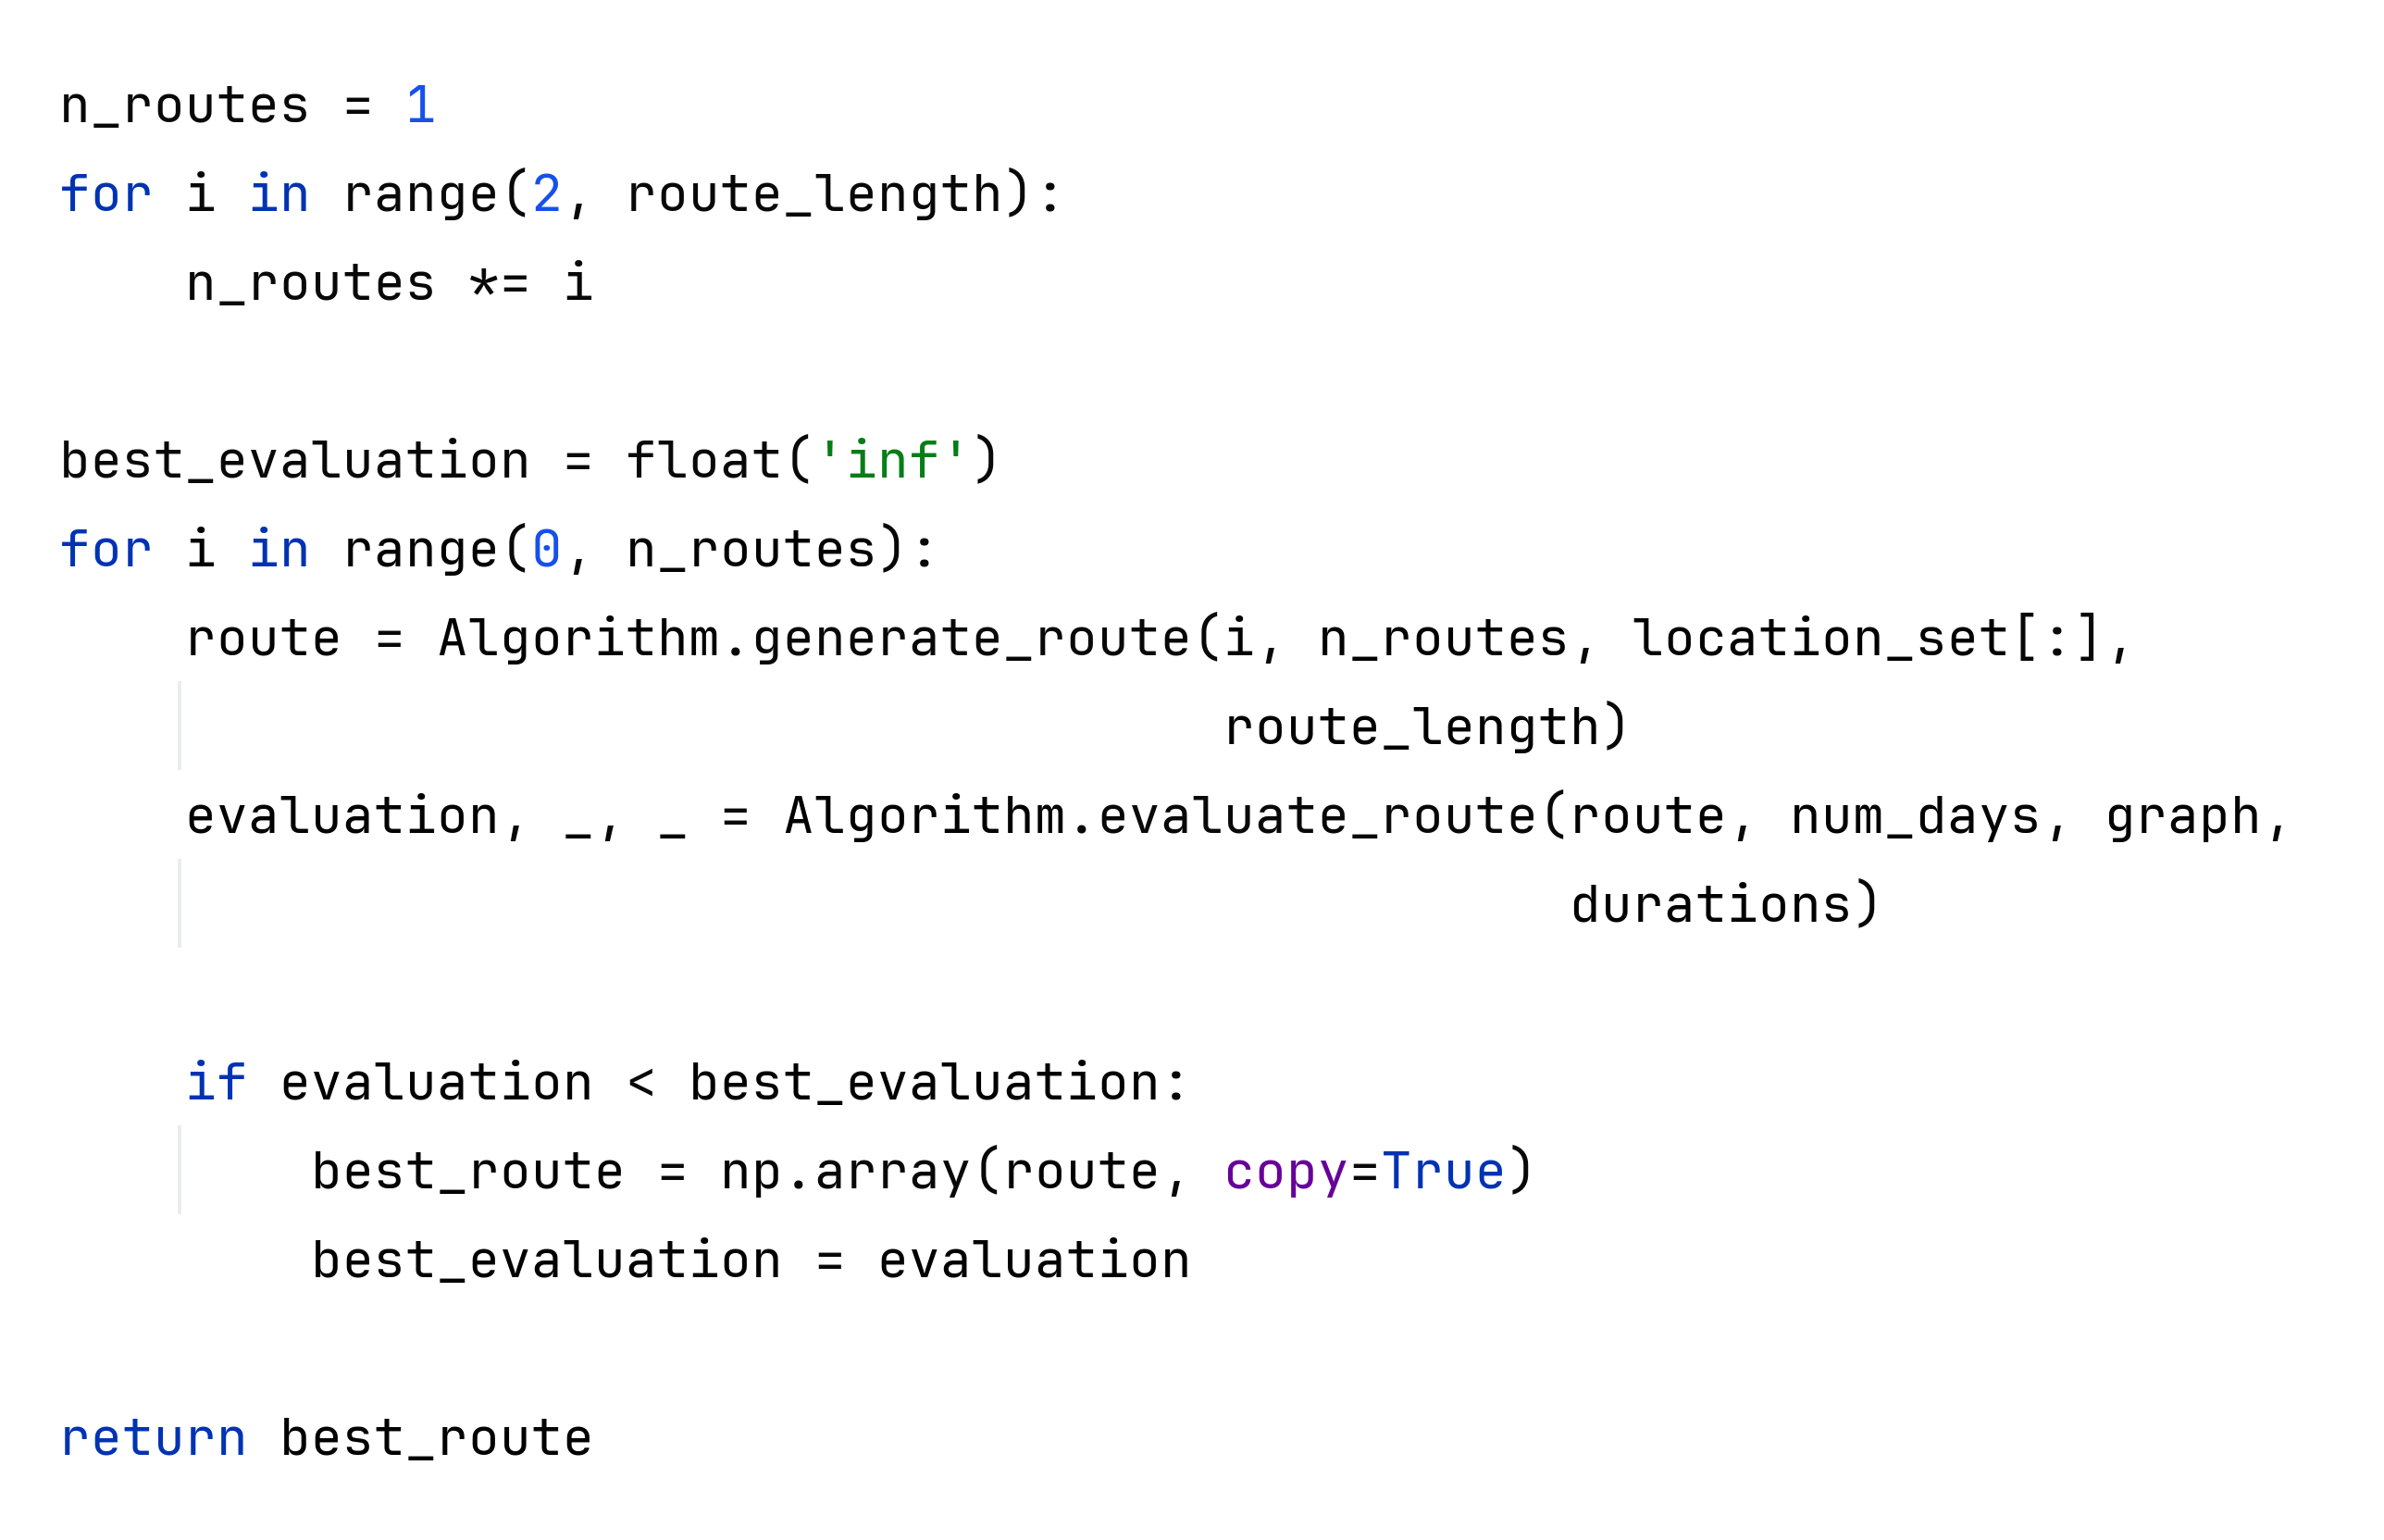
\includegraphics[width = \textwidth]{Routing.brute_force}
    \caption{Code from Routing.brute\_force in algorithms\textbackslash routing.py}
    \label{fig:Routing.brute_force}
\end{figure}

\noindent
Figure~\ref{fig:Bruteforce_Birmingham_Example} shows an example of the route find by performing Brute Force on an input
of 10 locations around Birmingham.
The location marked in green represents the starting point, and the blue marker indicates the first location
visited (showing the direction of the route).
\begin{figure}[H]
    \centering
    \includegraphics[width = \textwidth]{Bruteforce_Birmingham_Example}
    \caption{Example of a route found visiting 10 locations around Birmingham using Brute Force routing}
    \label{fig:Bruteforce_Birmingham_Example}
\end{figure}

\noindent
Being able to find a perfect route is certainly useful, but the computational cost of Brute Force becomes
impractical as the input size grows.
In calculating the 10 location route shown in figure~\ref{fig:Bruteforce_Birmingham_Example}, 362,880 possible routes
were considered, taking around 15 seconds.
If we were to use our maximum input size of 25 locations, over 620 sextillion routes would be considered \textemdash
which, assuming the same rate of routes evaluated per second, would take over 800 billion years.

Brute force was included in this project for its use as a benchmark.
Considering we will be evaluating algorithms based on their speed and the quality of their results, Brute Force offers
both an upper bound for quality and a lower bound for speed.

\subsubsection{Greedy Routing}\label{subsubsec:greedy-routing}
Greedy routing is a heuristic algorithm that builds a route iteratively, always choosing the next location according
to the shortest available path.
This is done by starting at the first location and then repeatedly selecting the next closest location until all
locations have been visited, then returning home.
At every location, we are checking the distance of every other location to find the closest, giving our greedy
algorithm a time complexity of $O(n^2)$.

\noindent
Greedy routing was by far the simplest algorithm to implement, and does not require much explanation.
For our implementation we will simply make a copy of our input, then iteratively find the closest locations.
When a location is visited, the edges leading to it are given an infinite cost to ensure that it is not visited again.
Our python implementation of greedy routing is shown in figure~\ref{fig:Routing.greedy_routing}.
\begin{figure}[H]
    \centering
    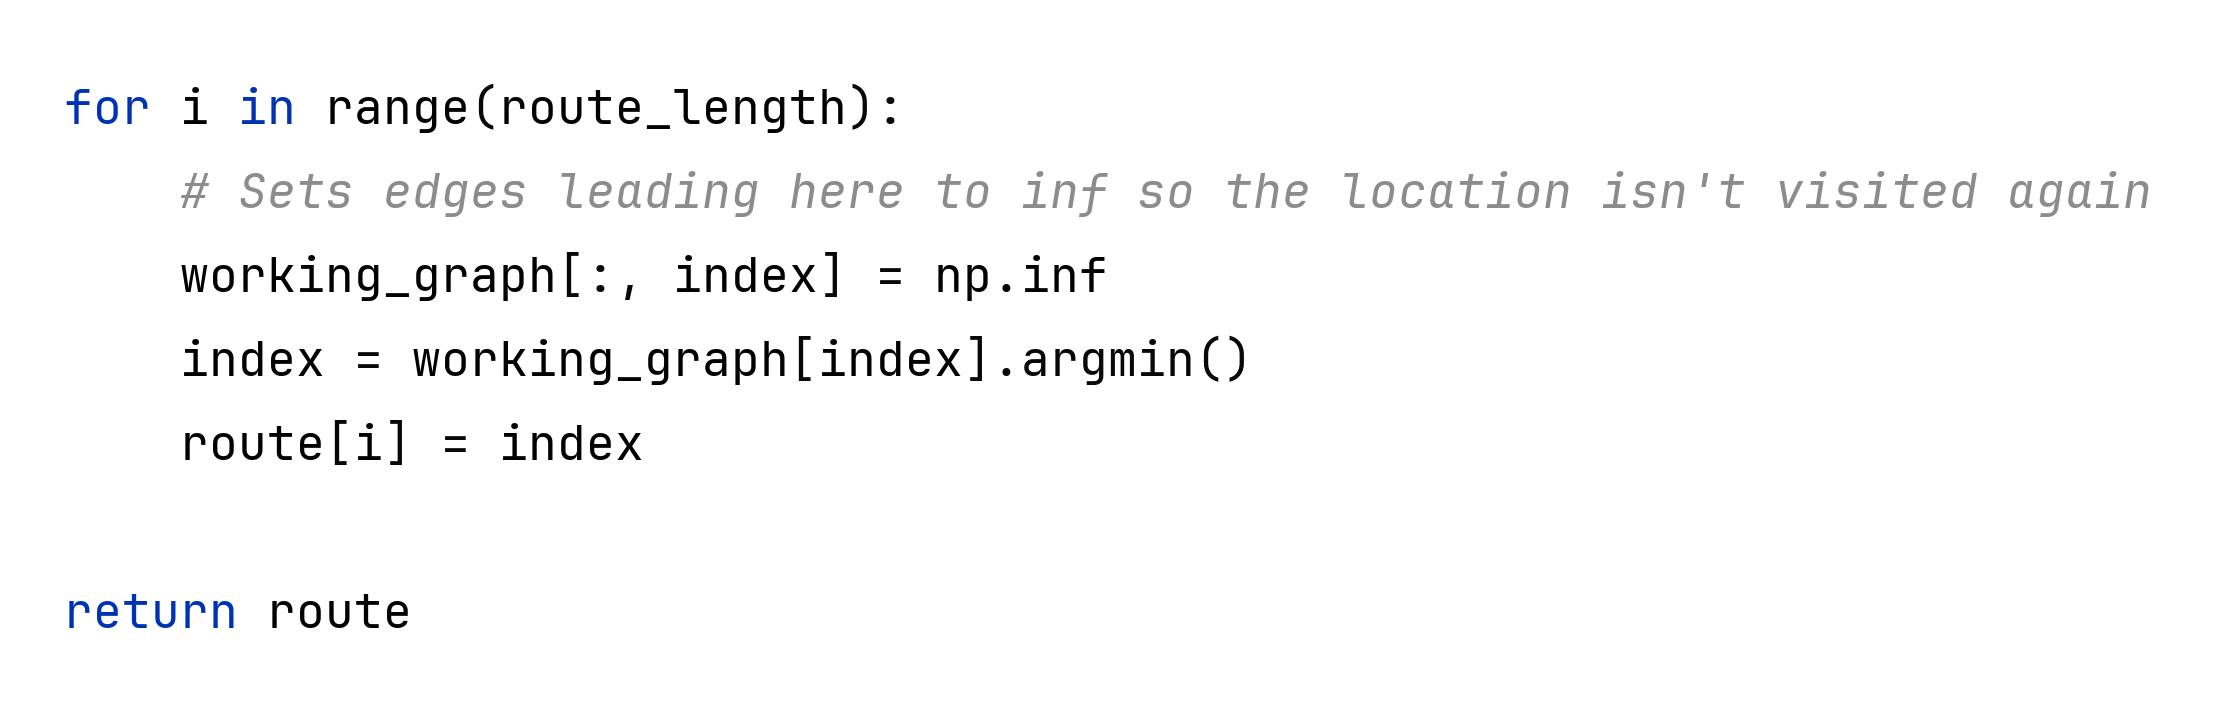
\includegraphics[width = \textwidth]{Routing.greedy_routing}
    \caption{Code from Routing.greedy\_routing in algorithms\textbackslash routing.py}
    \label{fig:Routing.greedy_routing}
\end{figure}

\noindent
Figure~\ref{fig:GreedyRouting_Birmingham_Example} shows an example of a route find by greedy routing, using the same
Birmingham input as that shown for Brute Force in figure~\ref{fig:Bruteforce_Birmingham_Example}.
\begin{figure}[H]
    \centering
    \includegraphics[width = \textwidth]{GreedyRouting_Birmingham_Example}
    \caption{Example of a route found visiting 10 locations around Birmingham using Greedy routing}
    \label{fig:GreedyRouting_Birmingham_Example}
\end{figure}

\noindent
As is perhaps evident from its example, greedy routing isn't always a great fit, with the effectiveness of the
algorithm being highly dependent on the input.
It may just happen that for some inputs the greedy algorithm will find a good route, but as input size grows and
routes become more complex, this becomes increasingly unlikely.

Where greedy routing does excell, and the reason for its inclusion in this project, is in its speed.
The algorithm found a route for the 10 location Birmingham input in less than a thousandth of a second, over 500,000
times faster than Brute Force.
Some fast routing algorithms are needed in order to use alongside our genetic clustering methods which, for
evaluation, require a route to be found for every individual in a population.

\subsubsection{Gift Wrapping}\label{subsubsec:gift-wrapping}
\todo{Explain gift wrapping algorithm}
\todo{Something like: "Once gift wrapping has found a convex hull, a greedy insertion algorithm is used to find the optimal route within the convex hull."}


\subsubsection{Genetic Routing}
\todo{Explain genetic routing}

\subsection{Route Insertion}\label{subsec:route-insertion}
\todo{Explain route insertion, how it is used in route planning and the goal of our algorithms.}
\subsubsection{Brute Force}\label{subsubsec:brute-force-route-insertion}
\todo{Explain how brute force algorithm can be modified for route insertion.}
\subsubsection{Greedy Insertion}\label{subsubsec:greedy-insertion}
\todo{Explain how greedy algorithm can be modified for route insertion.}

\subsection{Trip Generation}\label{subsec:trip-generation}
\todo{Explain trip generation, how it is used in route planning and the goal of our algorithms.}
\subsubsection{Brute Force}\label{subsubsec:brute-force-trip-generation}
\todo{Explain how brute force algorithm can be modified for trip generation.}
\subsubsection{Genetic Trip Generation}
\todo{Explain genetic trip generation}